% Generated from ../main.tex for Springer Nature submission-style compilation.
% Source of truth remains ../main.tex and ../content/*.tex.
\documentclass[pdflatex,sn-nature]{sn-jnl}

\usepackage[utf8]{inputenc}
\usepackage[T1]{fontenc}
\usepackage{graphicx}
\usepackage{booktabs}
\usepackage[htt]{hyphenat}
\usepackage{xurl}
\usepackage{amsmath}
\usepackage{amssymb}
\usepackage{longtable}
\usepackage{array}
\usepackage{caption}
\usepackage{float}
\usepackage{subcaption}
\usepackage{xcolor}
\usepackage{listings}
\usepackage[expansion=false]{microtype}
\usepackage{parskip}
\usepackage{seqsplit}
\usepackage{tcolorbox}
\tcbuselibrary{breakable}

\graphicspath{{../}{../../}}

\lstset{
  basicstyle=\small\ttfamily,
  breaklines=true,
  breakatwhitespace=false,
  frame=single,
  backgroundcolor=\color{gray!10},
  xleftmargin=1em,
  xrightmargin=1em,
}

\hypersetup{
  colorlinks=true,
  linkcolor=blue,
  urlcolor=blue,
  citecolor=blue,
}

\newcommand{\protocolstep}[2]{\par\medskip\noindent\textbf{#1 \textbar{} #2}\par}
\newcommand{\setupitem}[1]{\par\medskip\noindent\textbf{#1}\par}
\setcounter{secnumdepth}{0}
\raggedbottom

\makeatletter
\newcommand{\externalref}[2]{\@namedef{r@#1}{{#2}{0}{External reference}{Doc-Start}{}}}
\externalref{supp:analysis-of-published-datasets}{1}
\externalref{supp:comparison-delt-deli}{2}
\externalref{supp:enrichment-scores}{3}
\externalref{supp:enrichment-scores-comparison}{4}
\externalref{supp:reaction-graph-advanced}{5}
\externalref{tab:table11}{3}
\makeatother


\begin{document}

\title[DELT-Hit for DNA-encoded library analysis]{An end-to-end computational framework for DNA-encoded chemical library analysis}

\author*[1]{\fnm{Adriano} \sur{Martinelli}}\email{adriano.martinelli@pharma.ethz.ch}
\equalcont{These authors contributed equally to this work.}
\author[1]{\fnm{Alice} \sur{Lessing}}
\equalcont{These authors contributed equally to this work.}
\author[1]{\fnm{Gary} \sur{Hoppeler}}
\author[1]{\fnm{Leandro} \sur{Tollardo}}
\author[1]{\fnm{Johanna} \sur{Puff}}
\author[1]{\fnm{Andreas} \sur{Gloger}}
\author[1]{\fnm{Louise} \sur{Plais}}
\author*[1]{\fnm{J\"org} \sur{Scheuermann}}\email{joerg.scheuermann@pharma.ethz.ch}

\affil*[1]{\orgdiv{Institute of Pharmaceutical Sciences, Department of Chemistry and Applied Biosciences}, \orgname{ETH Zurich}, \orgaddress{\city{Zurich}, \postcode{8083}, \country{Switzerland}}}

\abstract{\noindent DNA-encoded chemical libraries (DELs) enable the screening of millions to billions of DNA-tagged small molecules
in a single experiment, with binders identified after PCR amplification and high-throughput DNA sequencing. Analysis of
DEL selection data requires the integration of sequence processing, cheminformatics, and statistical analysis, yet software
solutions supporting these steps are fragmented, limited in scope, or proprietary. This protocol describes DELT-Hit (DNA-Encoded Library Technology Hit Identification),
an open-source command-line tool for end-to-end DEL data analysis. DELT-Hit converts raw FASTQ reads into analysis-ready
chemical data through five connected modules: (i) sequence demultiplexing with error-tolerant barcode handling;
(ii) chemical structure reconstruction from building block libraries and reaction SMIRKS templates; (iii) molecular property
and descriptor calculation; (iv) enrichment analysis and hit ranking using count-based and RNA-seq-derived methods; and
(v) quality-control and visualization tools for DEL data interpretation. The workflow supports both single-display and
dual-display DEL architectures and produces standardized outputs for downstream analysis, including machine-learning applications.
Basic command-line skills are sufficient for routine analysis, whereas adapting SMIRKS for library enumeration workflows requires cheminformatics expertise.
Depending on library size, sequencing depth and hardware, the workflow typically requires one to several hours to complete. DELT-Hit is available at \url{https://github.com/DELTechnology/delt-hit}.}

\keywords{DNA-encoded chemical libraries, DEL analysis, cheminformatics, demultiplexing, enrichment analysis, open-source software}

\maketitle

\section*{Key points}

\begin{itemize}
  \item DELT-Hit supports the processing of industry-scale DEL datasets.
  \item Established tools such as Cutadapt and edgeR are integrated with DEL-specific sequence handling, enumeration, and quality control.
  \item The modular design supports diverse library formats including single-display and dual-display DEL architectures, custom reaction templates, and user-defined building block tables.
  \item Standardized outputs can be used directly for downstream cheminformatics and machine-learning analyses.
\end{itemize}

\section{Introduction}
DNA-encoded chemical libraries (DELs) enable the synthesis of billion-member compound collections and the screening of vast chemical spaces that would be difficult to access with conventional high-throughput screening\cite{brenner_encodedcombinatorialchemistry_1992,franzini_dnaencodedchemicallibraries_2014,favalli_dnaencodedchemicallibraries_2018,neri_dnaencodedchemicallibraries_2018,fitzgerald_dnaencodedchemistrydrug_2021,keller_impactdnaencodedchemical_2022,satz_dnaencodedchemicallibraries_2022,peterson_smallmoleculediscoverydnaencoded_2023,wichert_challengesprospectsdnaencoded_2024}. In analogy to biological display technologies, each library member is linked to an encoding DNA sequence, which connects phenotype (the small molecule) to genotype (the DNA tag). This design enables the parallel screening of very large libraries against biological targets and supports efficient hit discovery\cite{neri_dnaencodedchemicallibraries_2018,huang_strategiesdevelopingdnaencoded_2022}.

Affinity-based DEL selections can be automated and have been described previously in Nature Protocols\cite{decurtins_automatedscreeningsmall_2016}. After selection, the DNA tags of retained compounds are PCR-amplified and analyzed by high-throughput sequencing to determine the abundance of individual library members\cite{decurtins_automatedscreeningsmall_2016,satz_dnaencodedchemicallibraries_2022}. DELs are now used widely in both industry and academia\cite{satz_dnaencodedchemicallibraries_2022,peterson_smallmoleculediscoverydnaencoded_2023,wichert_challengesprospectsdnaencoded_2024,goodnow_dnaencodedchemistryenabling_2017}.

DEL architectures include single-display and dual-display formats, depending on whether the pharmacophore is presented on one DNA-linked fragment or on two pairing oligonucleotide strands\cite{lessing_advancingsmallmoleculedrug_2023}. Standard libraries are often encoded on double-stranded DNA headpieces, but single-stranded and Y-shaped encoding schemes are also used\cite{plais_universalencodingnext_2022}. Regardless of the encoding format, selection and PCR amplification ultimately produce double-stranded amplicons for DNA sequencing and downstream analysis\cite{decurtins_automatedscreeningsmall_2016}.

DEL datasets require the integration of sequence processing, cheminformatics, and statistical analysis, while offering unique opportunities for machine-learning-based modeling and discovery\cite{franzini_chemicalspacednaencoded_2016,mccloskey_machinelearningdnaencoded_2020,reiher_trendshittoleadoptimization_2021,shi_recentadvancesdnaencoded_2022,hou_machinelearningbaseddataanalysis_2023,shmilovich_deldockmoleculardockingenabled_2023,torng_deeplearningapproach_2023,edfeldt_datascienceroadmap_2024,edwards_proteinliganddata_2025,montoya_widespreadfalsenegatives_2025,sigel_dnaencodedlibrarymachine_2025,wang_rationaldesignstrategies_2025,gampe_analysesrecenthitfinding_2026}.
At the same time, DEL analysis poses challenges that are not addressed by standard genomics workflows, including demultiplexing complex barcode combinations, reconstructing chemical structures from encoded building blocks, comparing enrichment across conditions, and connecting selection outputs to downstream structure-based analysis.

Individual components of a DEL analysis workflow can be assembled from tools originally developed for cheminformatics and bioinformatics workflows, but these tools do not readily support the diversity of DEL architectures and experimental designs encountered in practice. In addition, they typically lack DEL-specific intermediate outputs and quality-control measures that facilitate troubleshooting, validation, and interpretation of results.


\subsection{Development of the protocol}
We developed DELT-Hit to support routine analysis of DEL campaigns across a wide range of library sizes and architectures.
The workflow combines and extends established tools and methods with DEL-specific sequence handling, chemical enumeration,
and quality control. Configuration files and standardized outputs support reproducibility, while the modular design allows
users to adapt the workflow to different experimental settings.


\begin{figure}[htbp]
\centering
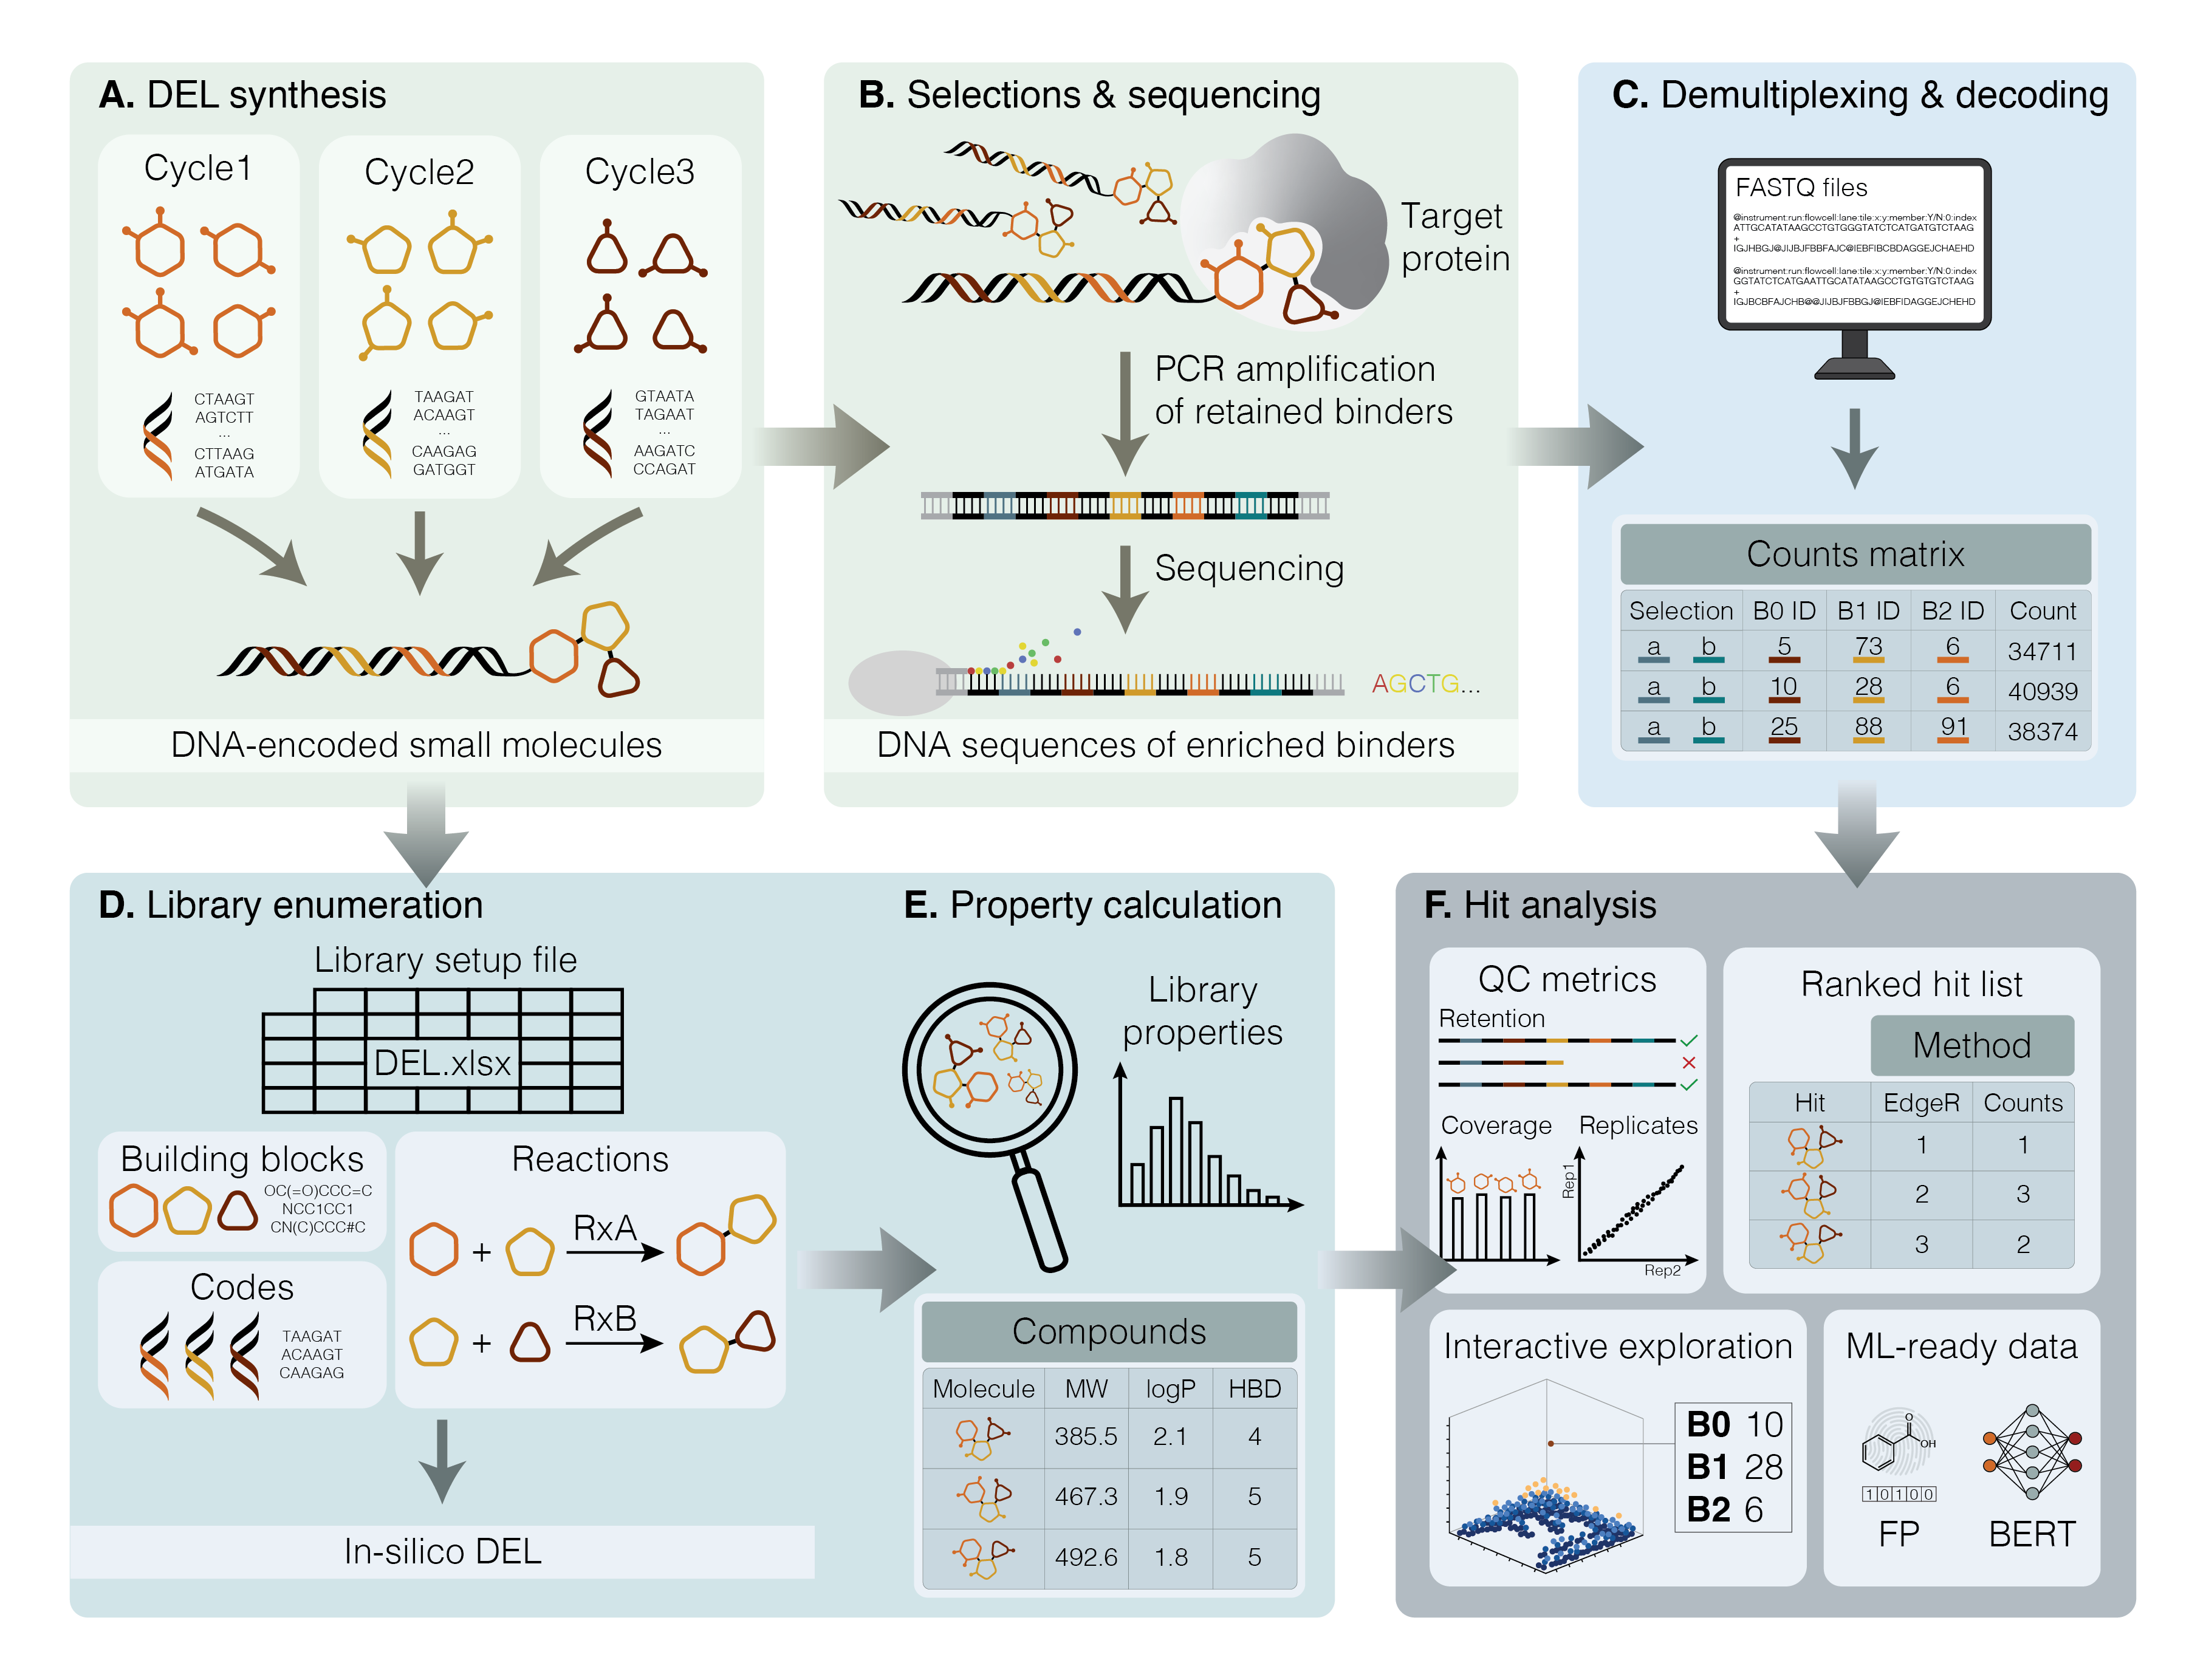
\includegraphics[width=\textwidth]{figures/workflow-overview.png}
\caption{DELT-Hit is organized into several modules (C - F) that complement the wet-lab DEL workflow (A - B). DEL synthesis (A) proceeds through iterative cycles of building block addition and encoding. Libraries are then screened in affinity-based selection experiments (B), after which retained DNA tags are PCR-amplified and sequenced. DELT-Hit uses Cutadapt\cite{martin_cutadaptremovesadapter_2011} to demultiplex sequencing reads (C) with user-defined error tolerances and produces count matrices for combinations of selection and building block codes. In parallel, library compounds can be enumerated in silico (D) from building block structures and reaction SMIRKS definitions, and molecular properties can be calculated (E). These in silico enumeration and property-calculation features can be applied before DEL synthesis to support library design and building-block selection. DELT-Hit subsequently integrates count data and chemical information for hit analysis (F), quality control, enrichment ranking, and interactive data exploration. In addition, the workflow exports molecular representations, including Morgan fingerprints and BERT embeddings, for downstream machine-learning applications.}
\label{fig:figure1}
\end{figure}
Figure~\ref{fig:figure1} summarizes the overall DELT-Hit workflow. The workflow integrates sequence demultiplexing via Cutadapt\cite{martin_cutadaptremovesadapter_2011}, chemical structure representation in SMILES\cite{weininger_smileschemicallanguage_1988,weininger_smiles2algorithm_1989,weininger_smiles3depict_1990}, reaction definitions in SMIRKS\cite{ref33,ref34} implemented in RDKit\cite{landrum_rdkitrdkit2025_09_4_2025}, different enrichment-analysis methods including edgeR\cite{robinson_edgerbioconductorpackage_2010}, molecular property calculation, library-member enumeration, and interactive visualization. Users can run the full workflow or individual modules, and each stage produces executable scripts and standardized outputs that can be adapted to more specialized analyses.


\subsection{Overview of the procedure}
The DELT-Hit protocol is organized into six analysis phases spanning 20 steps. Some downstream phases are optional or can be run independently:

(i) Project setup and library specification (Steps 1--9): Configuration file creation from Excel templates, library architecture definition, reaction specification, and experimental metadata setup.

(ii) Sequence demultiplexing and quality assessment (Steps 10--12): High-throughput sequencing data processing, barcode identification with error correction, and quality-control metric generation.

(iii) Data visualization and interpretation (Step 13): Interactive dashboard exploration of raw count data to identify selections of interest.

(iv) Selection enumeration and enrichment analysis (Steps 14--15): Automated SMILES generation and molecular property calculation for the top enriched compounds of a chosen selection.

(v) Statistical analysis and hit detection (Steps 16--17): Enrichment analysis using established RNA-seq methods, hit ranking with multiple statistical approaches, and result validation.

(vi) Full library enumeration and machine-learning representations (Steps 18--20): Optional full-library enumeration and generation of molecular fingerprints and embeddings for downstream machine-learning workflows.


\subsection{Applications of the method}
DELT-Hit accommodates library architectures ranging from simple two-cycle libraries to more complex multi-branch schemes. The workflow has been applied across several DEL campaigns:

A single-display DEL with two diversity elements comprising 366,600 glutamic acid derivatives (GB-DEL) was encoded in a single-display DNA format and tested in affinity-based selections, enabling de novo identification of binders against several pharmaceutically relevant proteins. The GB-DEL was also used for affinity maturation in a dual-display format by combining it with low-affinity hits displayed on a pairing strand\cite{bassi_singlestrandeddnaencodedchemical_2020}.

A second single-display DEL with two diversity elements comprising 670,752 derivatives based on a 2-azido-3-iodophenylpropionic acid scaffold (NF-DEL) was likewise encoded in a single-display DNA format and used to investigate the effect of stereo- and regiochemistry on ligand discovery. Selections against pharmaceutically relevant protein targets yielded selective enzyme inhibitors and binders to tumor-associated antigens that enabled conditional chimeric antigen receptor T-cell activation and tumor targeting\cite{favalli_stereoregiodefineddnaencoded_2021}.

A proof-of-principle single-display, double-stranded DEL containing 1,100 members and three amino acid diversity elements was synthesized on magnetic beads using a solid-phase approach with final release of the library from the support. The workflow supported analysis of both the standard released library and a self-purified version in which incomplete synthetic structures were removed before final release. Selections against carbonic anhydrase II and IX showed improved enrichment of the positive control for the self-purified DEL. Because synthesis and encoding yields correlate in this format, DNA sequencing of the unselected library can be used to assess chemical display yields. The solid-support synthesis also permits anhydrous reaction conditions and therefore enables water-free chemistry that is difficult to implement in standard DEL workflows\cite{keller_highlypurednaencoded_2024}.

A dual-display encoded self-assembling chemical (ESAC) library containing 56 million members enabled incremental connection of two displayed peptides. This library was used to study macrocycle flexibility with a two-step cyclization strategy. Selections against three targets revealed target-specific preferences for different conformational states, including a 314 nM thrombin inhibitor from the conformationally restrained macrocyclic subset, a more flexible streptavidin binder from the semi-closed conformation, and binders to human alkaline phosphatase (PLAP) from the open dual-display format\cite{petrov_flexibilitytuningdualdisplaydnaencoded_2025}.

The low- and medium-complexity studies presented here can be analyzed with DELT-Hit in less than 2 hours. Re-analyses of the published datasets from Favalli et al. and Keller et al. are summarized in Supplementary Note~\ref{supp:analysis-of-published-datasets}.

\subsection{Limitations}
While DELT-Hit addresses many challenges in DEL analysis, several limitations should be considered:

\begin{itemize}
  \item Computational complexity: Library size grows combinatorially with the number of diversity elements, primarily affecting library enumeration, property calculation, and molecular representation. In contrast, demultiplexing depends mainly on the number of sequencing reads (sequencing depth) and is therefore largely independent of library size. Although full enumeration of extremely large libraries can become computationally prohibitive, DELT-Hit supports selective enumeration of compounds detected in the individual selection experiments, substantially reducing computational requirements.
  \item Library chemistry: DELT-Hit supports arbitrary synthetic routes, provided that each route yields a single, well-defined final product. Libraries with non-standard reaction schemes, unconventional building block representations, or complex precursor handling may require additional configuration and validation. Accurate reaction SMIRKS definitions are essential for correct enumeration and require cheminformatics expertise.
\end{itemize}

\subsection{Comparison with other methods}

\newcommand{\statusgreen}{\raisebox{0.15ex}{\textcolor{green!50!black}{\LARGE$\bullet$}}}
\newcommand{\statusamber}{\raisebox{0.15ex}{\textcolor{orange!90!black}{\LARGE$\bullet$}}}
\newcommand{\statusopen}{\raisebox{0.15ex}{\textcolor{black!30}{\LARGE$\bullet$}}}
\newcommand{\statusred}{\raisebox{0.15ex}{\textcolor{blue!70!black}{\LARGE$\bullet$}}}
\begin{longtable}{p{8.8cm}>{\centering\arraybackslash}p{2.8cm}>{\centering\arraybackslash}p{1.2cm}}
\caption{Comparison of DELT-Hit and DELi\cite{wellnitz_opensourcednaencodedlibrary_2025} across selected scientific-software criteria. \statusgreen\ supported; \statusamber\ partial support; \statusopen\ not clearly documented; \statusred\ not supported.}
\label{tab:delt-deli-comparison} \\
\toprule
\textbf{Criterion} & \textbf{DELT-Hit} & \textbf{DELi} \\
\midrule
\endfirsthead

\toprule
\textbf{Criterion} & \textbf{DELT-Hit} & \textbf{DELi} \\
\midrule
\endhead

\multicolumn{3}{l}{\textbf{1. Workflow scope and usability}} \\
1.1 Library design support & \statusamber & \statusgreen \\
1.2 Configuration and workflow ergonomics & \statusgreen & \statusgreen \\
1.3 Interoperability and downstream reuse & \statusgreen & \statusamber \\
\midrule
\multicolumn{3}{l}{\textbf{2. Supported DEL architectures}} \\
2.1 Single-display support & \statusgreen & \statusgreen \\
2.2 Dual-display support & \statusgreen & \statusopen \\
\midrule
\multicolumn{3}{l}{\textbf{3. Decoding and sequencing-side QC}} \\
3.1 Error-tolerant demultiplexing & \statusgreen & \statusgreen \\
3.2 UMI-aware counting & \statusamber & \statusgreen \\
3.3 Decoding QC and reporting & \statusgreen & \statusgreen \\
\midrule
\multicolumn{3}{l}{\textbf{4. Chemical reconstruction and enumeration}} \\
4.1 Library enumeration & \statusgreen & \statusgreen \\
4.2 Flexible reaction-scheme support & \statusgreen & \statusred \\
\midrule
\multicolumn{3}{l}{\textbf{5. Statistical analysis and hit interpretation}} \\
5.1 Count-based enrichment & \statusgreen & \statusgreen \\
5.2 Statistical enrichment scoring & \statusgreen & \statusgreen \\
5.3 Synthon-level analysis & \statusred & \statusgreen \\
\midrule
\multicolumn{3}{l}{\textbf{6. Computational performance}} \\
6.1 Memory and scaling behavior & \statusgreen & \statusamber \\
\bottomrule
\end{longtable}

Pharmaceutical companies that run DEL campaigns typically use internal or licensed software platforms that integrate sequencing, barcode decoding, hit identification, and downstream prioritization within proprietary ecosystems. These systems can support scalability and automation, but they are closed-source and therefore limit methodological transparency, user-driven customization, and community-led improvement.

Contract research organizations (CROs) also provide DEL screening as a service against user-supplied targets. These services usually return processed results without exposing the underlying computational workflow or intermediate data products. As a result, users have limited opportunity to adapt the analysis, inspect intermediate outputs, or integrate DEL informatics into their own pipelines.

To our knowledge, DELi\cite{wellnitz_opensourcednaencodedlibrary_2025} is the only other open-source software package that combines barcode decoding, enrichment analysis, and library enumeration. DELi and DELT-Hit share several design principles, including modular architecture, transparent configuration, and integration with established bioinformatics and cheminformatics tools such as Cutadapt and RDKit (Table~\ref{tab:delt-deli-comparison}). DELT-Hit differs in several areas:

\begin{itemize}
  \item support for complex reaction paths,
  \item integration of RNA-seq-derived statistical models for hit calling that account for replicate structure and dispersion,
  \item support for widely used library designs, including single-display and dual-display formats.
\end{itemize}

DELT-Hit also exposes intermediate data products and executable scripts, allowing users to inspect, adapt, and extend each analysis step for reproducible benchmarking and integration. Furthermore, DELT-Hit exhibits substantially more favorable runtime and memory complexity than DELi, enabling the analysis of industry-scale libraries with billions of sequencing reads. A more detailed comparison of DELT-Hit and DELi is provided in Supplementary Note~\ref{supp:comparison-delt-deli}.

\section{Experimental Design}

\subsection{Input requirements}
DELT-Hit uses three main input categories. Library definition files in \texttt{.xlsx} format specify building block structures in SMILES format, reaction SMIRKS templates, DNA constant sequences, and barcode-to-building block mapping tables; these are typically provided as Excel workbooks with standardized sheet names for automated parsing. Raw sequencing data are supplied as \texttt{fastq.gz} or uncompressed FASTQ files generated by Illumina or compatible sequencing platforms. Experimental metadata are provided as \texttt{.yaml} files that define selection conditions, target proteins, control experiments, and replicate groupings for downstream statistical analysis and quality control. Table~\ref{tab:table1} summarizes these required inputs.

% BEGIN flattened input: tables/input-files
\begin{table}[htbp]
\centering
\caption{Input file specifications and sources}
\label{tab:table1}
\begin{tabular}{p{3.2cm}p{3.0cm}p{5.8cm}p{2.5cm}}
\toprule
File Type & Format & Description & Example Source \\
\midrule
Campaign definition & Excel (.xlsx) & Selection conditions, building blocks, reactions, and constants & Laboratory records \\
Sequencing data & FASTQ (.fastq / .fasta) & Raw sequencing reads & Illumina sequencer \\
Experimental metadata & YAML (.yaml) & Replicates used for enrichment analysis & Laboratory records \\
\bottomrule
\end{tabular}
\end{table}

% END flattened input: tables/input-files
\subsection{Command-line interface overview}
DELT-Hit is organized as a command-line workflow with dedicated commands for configuration generation, demultiplexing, library reconstruction, visualization, statistical analysis, and interactive inspection. Table~\ref{tab:delt-hit-api} summarizes the current user-facing CLI/API used throughout this protocol.

% BEGIN flattened input: tables/delt-hit-api
\begin{sidewaystable}
\centering
\small
\caption{Current DELT-Hit command-line API exposed by the user-facing CLI.}
\begin{tabular*}{\textheight}{@{\extracolsep\fill}p{2.2cm}p{2.8cm}p{6.4cm}p{3.8cm}}
\hline
\textbf{Group} & \textbf{Command} & \textbf{Purpose} & \textbf{Main outputs} \\
\hline
\texttt{init} & \texttt{delt-hit init} & Create a YAML experiment configuration from an Excel template. & \texttt{config.yaml} \\
\texttt{demultiplex} & \texttt{delt-hit demultiplex prepare} & Generate Cutadapt input files and a shell script for barcode parsing. & Cutadapt input files, \texttt{demultiplex.sh} \\
\texttt{demultiplex} & \texttt{delt-hit demultiplex process} & Parse demultiplexed reads and compute per-selection barcode counts. & Per-selection \texttt{counts.txt} tables \\
\texttt{demultiplex} & \texttt{delt-hit demultiplex report} & Summarize Cutadapt and demultiplexing statistics. & QC text report \\
\texttt{demultiplex} & \texttt{delt-hit demultiplex qc} & Generate quality-control plots from demultiplexed counts. & QC plots \\
\texttt{library} & \texttt{delt-hit library enumerate} & Enumerate the DEL from the reaction graph and generate compound SMILES. & Library parquet, optional debug reaction-graph PNGs \\
\texttt{library} & \texttt{delt-hit library properties} & Compute molecular descriptors for an enumerated library. & Properties parquet, descriptor histograms \\
\texttt{library} & \texttt{delt-hit library represent} & Generate machine-learning representations such as Morgan fingerprints. & Sparse representation matrix (\texttt{.npz}) \\
\texttt{visualize} & \texttt{delt-hit visualize enumerate} & Render reaction graphs, reaction schemes, building blocks, and configured compounds. & Chemistry visualization PNGs \\
\texttt{visualize} & \texttt{delt-hit visualize library} & Render 2D structure panels for compounds in a named library. & Per-compound library PNGs \\
\texttt{analyse} & \texttt{delt-hit analyse enrichment} & Run enrichment analysis from count tables using count-based or edgeR-based workflows. & Enrichment result tables and normalized counts \\
\texttt{dashboard} & \texttt{delt-hit dashboard} & Launch an interactive Dash application to inspect a selection's count data. & Local web dashboard \\
\hline
\end{tabular*}
\label{tab:delt-hit-api}
\end{sidewaystable}

% END flattened input: tables/delt-hit-api
\subsection{Library architecture considerations}
DELT-Hit supports several library architectures, including single-display libraries with linear synthetic schemes in which DNA tags are appended after each reaction cycle as well as dual-display libraries in which compounds are presented on both complementary DNA strands. More complex multi-cycle libraries with branching reactions and multiple building block incorporation sites are also supported.


\subsection{Library chemistry and reaction definition}
Reaction cycles used during library construction are specified as reaction SMIRKS in the Excel configuration file. DELT-Hit translates these definitions into an explicit reaction graph capable of representing diverse library architectures, including multiple reaction cycles, branching pathways, and multi-step transformations. This flexibility allows the analysis of a wide range of DEL designs, provided that each synthetic route resolves to a single, well-defined final product.

Libraries with non-standard reaction schemes, unconventional building block representations, or complex precursor handling may require additional customization and validation. Because library enumeration relies on accurate SMIRKS definitions, DELT-Hit provides templates for commonly used DEL reactions (see Supplementary Notes), but library-specific adaptations require cheminformatics expertise to ensure chemically correct product formation and reliable structure reconstruction. 


\subsection{Quality control parameters}
DELT-Hit monitors several quality metrics throughout the workflow. These include demultiplexing efficiency, defined as the proportion of sequencing reads assigned to valid barcode combinations and typically exceeding 70\% in high-quality datasets; barcode recovery rates, which can help identify technical artifacts or configuration errors; statistical significance measures based on multiple-testing correction and false-discovery-rate control using established methods for count-based sequencing data; consistency across biological and technical replicates; and reaction validation to confirm that the specified reaction definitions generate the expected chemical products.


\subsection{Project initialization and configuration}

DELT-Hit uses a YAML configuration file that defines library structure, experimental design, and analysis parameters. This file is produced from a standardized Excel template that contains the DEL and experimental design information. The protocol guides users through the creation and completion of this workbook in the Procedure section. The Excel sheets and their respective contents and functions are explained here. 

The \texttt{experiment} sheet contains the experiment name, file paths, and computational resource settings. 

The \texttt{selection} sheet defines the experimental design, including selection conditions, multiplexing barcodes, and replicate grouping. Each row describes one experimental setting, such as a target condition or control condition, and is identified by a unique combination of \texttt{S0} and \texttt{S1} primers for demultiplexing. 

The \texttt{structure} sheet defines the DNA construct architecture and error tolerances for demultiplexing. Each DNA region is identified by a unique name. A \texttt{max\_error\_rate} and the allowance of indels can be configured separately for each region. The \texttt{reverse} and \texttt{complement} flags control optional codon orientation transforms during matching and are mostly relevant for dual-display libraries. An example dual-display workbook illustrating the dual-display-specific columns is provided in the DELT-Hit GitHub repository under \texttt{supporting\_material/experiments/example-dual-display/}. 

The \texttt{constant} sheet contains the DNA sequences for all constant regions defined in the \texttt{structure} sheet. 

The \texttt{building block} sheets contain the coding information and chemical structures of all encoded building blocks and indicate the reactions to which they are subjected during library synthesis. DELT-Hit supports libraries with an arbitrary number of building block regions. A separate \texttt{building block} sheet is required for each barcode region defined in the structure sheet. 

The \texttt{reactions} sheet defines all chemical reactions used during library synthesis with SMIRKS notation\cite{ref34} and is only required for library enumeration. Although reaction templates commonly employed in DEL synthesis are provided in the Supplementary Notes, customization by the user may be required depending on the library setup and the building blocks employed. Before attempting to enumerate an entire library, we recommend validating all reaction notations with a representative subset of building blocks. If the same reaction type is used at multiple stages of the synthesis, each instance must be defined as a separate reaction.

The \texttt{compounds} sheet is only required for library enumeration and is used to define any additional chemical compounds (scaffolds, reactants) used during library synthesis. 

The \texttt{reaction graph} sheet allows advanced library enumeration with additional steps such as precursor conversion or deprotection reactions. More advanced reaction-graph edge cases, including multi-path precursor activation schemes that require separate reaction nodes, are described in Supplementary Note~\ref{supp:reaction-graph-advanced}; a concrete two-path precursor-activation example is summarized in Supplementary Table~\ref{tab:table11}. 

Once the Excel file is completed with all required sheets, the YAML configuration file can be generated. 

\subsection{Sequence processing and demultiplexing}

DELT-Hit uses Cutadapt to process raw sequencing reads according to the demultiplexing parameters defined in the Excel file. This enables the identification and counting of each library member in the selection experiments. Users can decide to allow insertions/deletions during barcode matching (\texttt{indels} in the \texttt{structure} sheet) and set the tolerance for sequencing errors (\texttt{max\_error\_rate} in the \texttt{structure} sheet). The demultiplexing process performs adapter detection and trimming, sequential extraction of selection and building-block barcodes, and quality filtering of reads that exceed the defined error thresholds. The generated shell script runs Cutadapt on the FASTQ file and maps reads to selection and codon identifiers. It produces \texttt{reads\_with\_adapters.gz}, which contains all mapped sequences. After demultiplexing, a report of read retention across demultiplexing stages and QC figures are generated. These allow the user to inspect whether the read retention and barcode recovery are sufficient to proceed. If the quality-control inspection is satisfactory, the demultiplexed reads can be aggregated into selection-level count tables. DELT-Hit does this by parsing the demultiplexed reads, mapping barcode combinations to library members, and finally generating count tables for each selection. The results are saved in a standardized format. 

\subsection{Data visualization and interpretation}

Once sequence processing and demultiplexing is complete, DELT-Hit provides various ways to visualize and analyze selection results. The dashboard displays experimental metadata, including selection conditions, target information, and experimental parameters, along with scatter plots for the selected condition. Users can switch between count files, inspect aggregated counts across codon dimensions, and apply filters to focus on specific regions of the count distribution. While the dashboard displays raw counts from demultiplexing, the statistical analysis and hit identification section enables statistical comparisons and hit identification based on enrichment analysis. 

\subsection{Selection enumeration and enrichment analysis}

DELT-Hit supports selection-based compound enumeration for streamlined evaluation of enriched library members. Given a user-defined threshold \texttt{top\_n}, the workflow first enumerates the most enriched compounds in the selected experiment, generating their chemical structures. For easier visualization, a reaction graph, corresponding reaction schemes, and catalogs of 2D molecular representations of both the building blocks and enumerated compounds are also generated. In a second step, molecular descriptors are computed to characterize the chemical space of the enumerated compounds. These include Lipinski descriptors such as molecular weight (MW), partition coefficient (LogP) or hydrogen-bond donors (HBD).

\subsection{Statistical analysis and hit identification}

DELT-Hit implements methods to identify enriched library members by comparing results obtained from different selection conditions. A dedicated analysis configuration file based on the information from the \texttt{selection} sheet can be generated by the user to specify which selections to compare. The configuration defines the comparisons to be performed across selection runs, including runs derived from multiple sequencing files. Each \texttt{experiment} entry specifies a single named comparison and contains a list of \texttt{selections} for the comparison. Each entry within the \texttt{selections} list can be attributed to either a control or condition \texttt{group}. 

DELT-Hit supports three statistical approaches for identifying enriched compounds. All methods generate an R script that can be executed directly or adapted further by the user to fit more specialized workflows. A simple count-based method and edgeR are designed for evaluation settings with replicates, whereas the normalized z-score method can also be used for experiments without replicates.

% Method A (simple counts method) averages counts across replicates within each group and computes a direct enrichment score from the difference between the condition and control groups. It does not provide formal significance testing, but it is useful as a straightforward ranking approach when replicate-based comparisons are being evaluated.

% Method B (edgeR method) applies RNA-seq-derived statistical modeling with empirical Bayes shrinkage, reports false-discovery-rate-corrected \textit{P} values, and provides normalized count tables for each selection. It requires replicates and is best used as a significance-annotation layer alongside enrichment ranking.

% Method C (normalized z-score method) computes the per-compound score for an individual selection following Faver et al.\cite{faver_quantitativecomparisonenrichment_2019}. In the current implementation, the generated output contains both the raw \texttt{z\_score} and the depth-normalized \texttt{norm\_z\_score}, defined as $z\_score / \sqrt{n}$ and used for ranking. Because this approach does not rely on replicate-based variance estimation, it can also be applied to experiments without replicates.

A comparison of enrichment score rankings for recovery of a previously reported CAIX-associated building block by Favalli \cite{favalli_stereoregiodefineddnaencoded_2021} is provided in Supplementary Note~\ref{supp:enrichment-scores-comparison}, and the underlying statistical definitions are summarized in Supplementary Note~\ref{supp:enrichment-scores}.

\subsection{Full library enumeration and machine learning representations}

While selection-based compound enumeration enables rapid analysis of library-member subsets, DELT-Hit also supports full-library enumeration. Although this is computationally much more expensive than the focused approach, it can be useful for downstream machine-learning applications and can support evaluation of prospective libraries with respect to their properties while informing building-block selection even before DEL synthesis. Full-library enumeration generates molecular representations for all library compounds and computes their molecular properties. To prepare for downstream machine-learning applications, DELT-Hit supports the generation of two types of molecular representations compatible with common machine-learning frameworks. Morgan circular fingerprints (2048-bit vectors) are useful for similarity searching and clustering and can be created using the \texttt{morgan} method implemented in DELT-Hit. For deep-learning applications, the \texttt{bert} method allows the creation of transformer-based molecular embeddings (768-dimensional vectors). Both representations are compatible with scikit-learn, PyTorch, and TensorFlow.

\section{Materials}

\subsection{Equipment}
Hardware:

\begin{itemize}
  \item Minimum configuration: 16 GB RAM, 8 CPU cores, 50 GB available storage
  \item Recommended configuration: 32 GB RAM, 16 CPU cores, 100 GB available storage
  \item High-performance setup: 64 GB RAM, 32 CPU cores, 250 GB SSD storage
  \item Operating systems: Linux (Ubuntu 20.04+), macOS (12.0+), and Windows 10/11 (with Windows Subsystem for Linux recommended)
\end{itemize}

\subsection{Software dependencies}
Core requirements are:

\begin{itemize}
  \item Python 3.12 or higher with pip package manager
  \item Conda package manager (Miniconda or Anaconda)
  \item R statistical computing environment (version 4.1+)
\end{itemize}
Python packages:

\begin{itemize}
  \item cutadapt (4.9+): Sequence adapter trimming and demultiplexing
  \item rdkit (2024.3+): Chemical structure processing and property calculation
  \item pandas (2.2+): Data manipulation and statistical analysis
  \item numpy (1.24+): Numerical computing and array operations
  \item matplotlib/seaborn: Data visualization and publication-quality plotting
  \item plotly: Interactive visualization and dashboard components
  \item scipy (1.10+): Statistical functions and optimization algorithms
\end{itemize}
R packages:

\begin{itemize}
  \item edgeR: Differential expression analysis adapted for count data
  \item limma: Linear modeling and empirical Bayes statistics
  \item tidyverse: Data manipulation and visualization tools
  \item GGally: Extension to ggplot2 for correlation matrices
  \item BiocManager: Bioconductor package management
\end{itemize}

\subsection{Data}
We provide a complete single-display DELT-Hit example dataset to demonstrate the full workflow from initialization through demultiplexing, library reconstruction, and enrichment analysis. A complementary dual-display example focused on library enumeration and visualization is also included in the supporting material. The example is based on the architecture of a published library\cite{bassi_singlestrandeddnaencodedchemical_2020} and can be accessed through the repository's supporting material.
The dataset includes \texttt{example-single-display.xlsx}, which defines the library architecture and experimental setup; \texttt{campaign.fastq.gz}, which contains representative sequencing reads from the screen; and \texttt{analysis.yaml}, which specifies the comparisons used for hit identification. The files \texttt{example-single-display.xlsx} and \texttt{analysis.yaml} are available in the GitHub repository under \path{supporting_material/experiments/example-single-display/}. Table~\ref{tab:table2} lists the tutorial inputs and persistent archives. A complete end-to-end walkthrough of this example is provided in Box~2 in the Procedure.

% BEGIN flattened input: tables/tutorial-datasets
\begin{table}[htbp]
\centering
\caption{Tutorial datasets for protocol validation}
\label{tab:table2}
\begin{tabular}{p{4.0cm}p{6.5cm}p{4.0cm}}
\toprule
File & URL & Description \\
\midrule
campaign.fastq.gz & \url{https://ndownloader.figshare.com/files/61487743} & Representative screening data for the single-display example \\
example-single-display.xlsx & \path{supporting_material/experiments/example-single-display/} & Complete library and experimental definitions for the full single-display workflow \\
analysis.yaml & \path{supporting_material/experiments/example-single-display/} & Experiment configuration for enrichment analysis \\
Full workflow archive & \url{https://doi.org/10.5281/zenodo.20447074} & Persistent archive containing the single-display workflow data together with generated outputs \\
Code release archive & \url{https://doi.org/10.5281/zenodo.20556531} & Persistent archive of the DELT-Hit code release used to produce the workflow outputs \\
\bottomrule
\end{tabular}
\end{table}

% END flattened input: tables/tutorial-datasets
\begin{tcolorbox}[
  colback=gray!10,
  colframe=gray!50,
  title=Box 1 | Installing DELT-Hit,
  fonttitle=\bfseries
]

\setupitem{Environment setup with Conda}

We recommend using Miniconda to create an isolated environment with controlled dependencies. This step is only required once.


\begin{lstlisting}
# Download and install Miniconda for your operating system
# Follow instructions at: https://docs.anaconda.com/miniconda

# Create dedicated environment (only needed once)
conda create -n delt-hit python=3.12 -y

# Activate environment (required for each new terminal session)
conda activate delt-hit
conda install pygraphviz -y

# Install DELT-Hit package
pip install git+https://git@github.com/DELTechnology/delt-hit.git
\end{lstlisting}
<CRITICAL>: Activate the \texttt{delt-hit} conda environment using \texttt{conda activate delt-hit} each time you open a new terminal session before running DELT-Hit commands. We also recommend initializing the shell with Conda during installation so that the \texttt{conda} command is available in new terminal windows. 


\setupitem{R environment configuration}

Statistical analysis requires R and specific Bioconductor packages. This configuration is only required once. Open R or RStudio and execute:


\begin{lstlisting}
# Install required CRAN packages
install.packages(c("tidyverse", "GGally"))

# Install BiocManager for Bioconductor packages
if (!require("BiocManager", quietly = TRUE))
    install.packages("BiocManager")

# Install Bioconductor packages
BiocManager::install(c("edgeR", "limma"))
\end{lstlisting}

\setupitem{Installation verification}

Verify that all components are correctly installed:


\begin{lstlisting}
# Activate environment
conda activate delt-hit

# Test core functionality
delt-hit --help

# Expected output: Help message describing the delt-hit command
\end{lstlisting}

\textbf{$\blacklozenge$ Troubleshooting}

\end{tcolorbox}
\clearpage

\subsection{Experimental setup}
The installation procedure detailed in Box~1 is performed once before running the DELT-Hit workflow. Subsequent analyses are executed from the command line within the same software environment.

\section{Procedure}

\begin{tcolorbox}[
  colback=blue!5,
  colframe=blue!40,
  breakable,
  title=Box 2 | Quickstart: single-display example workflow,
  fonttitle=\bfseries
]

The following workflow reproduces the complete DELT-Hit analysis for the single-display example dataset provided in the supporting material (see Section~3.3 Data). It is intended as a self-contained reference for users who want to run through the entire pipeline on the provided example before adapting it to their own data. This workflow produces the outputs presented in the Anticipated Results section. DELT-Hit needs to be installed as described in Box~1.

\setupitem{Download the repository and enter the example directory}

\begin{lstlisting}
git clone https://github.com/DELTechnology/delt-hit.git
cd delt-hit/supporting_material/experiments/example-single-display
\end{lstlisting}

\setupitem{Download the example data}

\begin{lstlisting}
cd supporting_material/experiments/example-single-display
bash download.sh
\end{lstlisting}

\setupitem{Initialize the configuration}

\begin{lstlisting}
delt-hit init --excel_path=example-single-display.xlsx
CONFIG_PATH=campaign/config.yaml
ANALYSIS_CONFIG_PATH=analysis.yaml
ANALYSIS_OUTPUT_ROOT=campaign/analysis
\end{lstlisting}

\setupitem{Demultiplexing}

\begin{lstlisting}
delt-hit demultiplex prepare --config_path="$CONFIG_PATH"
bash campaign/demultiplex/cutadapt_input_files/demultiplex.sh
delt-hit demultiplex report --config_path="$CONFIG_PATH"
delt-hit demultiplex qc --config_path="$CONFIG_PATH"
delt-hit demultiplex process --config_path="$CONFIG_PATH"
delt-hit demultiplex process --config_path="$CONFIG_PATH" --as_files=True
\end{lstlisting}

\setupitem{Library enumeration and visualization}

\begin{lstlisting}
delt-hit visualize enumerate --config_path="$CONFIG_PATH"
delt-hit library enumerate \
  --config_path="$CONFIG_PATH" \
  --counts_path=campaign/selections/AG24_4/counts.txt \
  --top_n=1000 \
  --library_name=AG24_4_top_hits
delt-hit visualize library --config_path="$CONFIG_PATH" \
  --library_name=AG24_4_top_hits
delt-hit library properties --config_path="$CONFIG_PATH" \
  --library_name=AG24_4_top_hits
delt-hit dashboard \
  --config_path="$CONFIG_PATH" \
  --counts_path=campaign/selections/AG24_4/counts.txt
\end{lstlisting}

\setupitem{Enrichment analysis}

\begin{lstlisting}
delt-hit analyse enrichment \
  --analysis_config="$ANALYSIS_CONFIG_PATH" \
  --name=condition_vs_control --method=counts \
  --save_dir="$ANALYSIS_OUTPUT_ROOT"
Rscript --vanilla "$ANALYSIS_OUTPUT_ROOT/counts/condition_vs_control/enrichment_counts.R"

delt-hit analyse enrichment \
  --analysis_config="$ANALYSIS_CONFIG_PATH" \
  --name=condition_vs_control --method=edgeR \
  --save_dir="$ANALYSIS_OUTPUT_ROOT"
Rscript --vanilla "$ANALYSIS_OUTPUT_ROOT/edgeR/condition_vs_control/enrichment_edgeR.R"

for selection in AG24_13 AG24_14 AG24_15; do
  delt-hit analyse enrichment \
    --config_path="$CONFIG_PATH" \
    --counts=campaign/selections/$selection/counts.txt \
    --method=z_score --name=$selection \
    --save_dir="$ANALYSIS_OUTPUT_ROOT"
  Rscript --vanilla "$ANALYSIS_OUTPUT_ROOT/z_score/$selection/enrichment_z_score.R"
done
\end{lstlisting}

\setupitem{Full library enumeration and molecular representations}

\begin{lstlisting}
delt-hit library enumerate --config_path="$CONFIG_PATH"
delt-hit library properties --config_path="$CONFIG_PATH"
delt-hit library represent --method=morgan --config_path="$CONFIG_PATH"
delt-hit library represent --method=bert --config_path="$CONFIG_PATH"
\end{lstlisting}

\end{tcolorbox}

\subsection{Phase 1 | Project initialization and configuration}

\textbf{TIMING:} 15--60 min

<CRITICAL>: In this phase, a YAML configuration file is created from an Excel workbook that contains the DEL and experimental design information. The following steps describe the required sheets and their format. We recommend starting from the example workbook provided on GitHub (under \texttt{templates}) and adjusting it to the new library.


\protocolstep{1}{Create the experiment sheet}

Table~\ref{tab:table3} shows the complete layout of the \texttt{experiment} sheet. Required fields of the \texttt{experiment} sheet are as follows: 

\begin{itemize}
  \item \texttt{name}: Experiment name
  \item \texttt{fastq\_path}: File path
  \item \texttt{save\_dir}: Directory under which DELT-Hit outputs are written, created as \texttt{\textless save\_dir\textgreater/\textless name\textgreater}
  \item \texttt{num\_cores}: Defines the number of CPU cores used for the demultiplexing step
\end{itemize}

% BEGIN flattened input: tables/experiment-config
\begin{table}[htbp]
\centering
\caption{Experiment configuration parameters}
\label{tab:table3}
\begin{tabular}{ll}
\toprule
variable & value \\
\midrule
name & campaign \\
fastq\_path & campaign.fastq.gz \\
save\_dir & ./ \\
num\_cores & 11 \\
\bottomrule
\end{tabular}
\end{table}

% END flattened input: tables/experiment-config
<CRITICAL> Use absolute paths, or paths relative to the working directory, for \texttt{fastq\_path} and \texttt{save\_dir}. Here, \texttt{./} refers to the current working directory from which the command is run.


\protocolstep{2}{Create the selection sheet}

Define the experimental design within this sheet, including selection conditions, multiplexing barcodes, and replicate grouping. Table~\ref{tab:table4} shows an example layout. Required columns for demultiplexing:

\begin{itemize}
  \item \texttt{name}: Unique identifier for each selection
  \item \texttt{S0}, \texttt{S1}: Multiplexing barcodes for selection identification
\end{itemize}
Optional columns:

\begin{itemize}
  \item \texttt{group}: Statistical grouping when needed for downstream analyses (for example, "condition" or "control")
  \item \texttt{operator}: Person who performed the selection
  \item \texttt{date}: Date of selection experiment
  \item Other columns can be added at the user's discretion
\end{itemize}

% BEGIN flattened input: tables/selection-design
\begin{table}[htbp]
\centering
\caption{Selection experimental design}
\label{tab:table4}
\begin{tabular}{lllllll}
\toprule
name & operator & date & group & target & S0 & S1 \\
\midrule
AG24\_4 & A. Smith & 26-Sep-24 & control &  & ACACAC & TCGATA \\
AG24\_5 & A. Smith & 26-Sep-24 & control &  & ACAGCA & TCGATA \\
AG24\_6 & A. Smith & 26-Sep-24 & control &  & ACATGT & TCGATA \\
AG24\_13 & A. Smith & 26-Sep-24 & condition & A & ACGACG & TCGATA \\
AG24\_14 & A. Smith & 26-Sep-24 & condition & A & ACGCGA & TCGATA \\
AG24\_15 & A. Smith & 26-Sep-24 & condition & A & ACTAGC & TCGATA \\
\bottomrule
\end{tabular}
\end{table}

% END flattened input: tables/selection-design
\protocolstep{3}{Create the structure sheet}

Define the DNA construct architecture and error tolerances for demultiplexing. Each DNA region is identified by a unique name across three types of DNA regions:

\begin{itemize}
  \item \texttt{selection}: Region used for selection primers defined in the \texttt{selection} sheet. These regions should be named \texttt{S0} and \texttt{S1}.
  \item \texttt{constant}: Constant regions shared across DNA constructs. These regions should be named sequentially \texttt{C0}, \texttt{C1}, ..., \texttt{CN}.
  \item \texttt{building\_block}: Region identifying a chemical building block. These regions should be named sequentially \texttt{B0}, \texttt{B1}, ..., \texttt{BN}.
\end{itemize}

Table~\ref{tab:table5} summarizes the expected layout. The following columns and parameters are to be defined: 

\begin{itemize}
  \item \texttt{name}: Unique identifier for each DNA region
  \item \texttt{type}: Region type (\texttt{selection}, \texttt{constant}, or \texttt{building\_block})
  \item \texttt{max\_error\_rate}: Maximum allowed error rate for adapter trimming (0 = perfect match, 0.1 = 10\% errors), configured separately for each region
  \item \texttt{indels}: Whether to allow insertions/deletions (\texttt{TRUE}/\texttt{FALSE})
  \item \texttt{reverse}: Whether to reverse the codon before matching (\texttt{TRUE}/\texttt{FALSE}; mostly relevant for dual-display libraries)
  \item \texttt{complement}: Whether to complement the codon before matching (\texttt{TRUE}/\texttt{FALSE}; mostly relevant for dual-display libraries)
\end{itemize}

% BEGIN flattened input: tables/sequence-structure
\begin{table}[htbp]
\centering
\caption{DNA sequence structure definition}
\label{tab:table5}
\begin{tabular}{llllll}
\toprule
name & type & max\_error\_rate & indels & reverse & complement \\
\midrule
S0 & selection & 0 & FALSE & FALSE & FALSE \\
C0 & constant & 1.01 & FALSE & FALSE & FALSE \\
B0 & building\_block & 0 & FALSE & FALSE & FALSE \\
C1 & constant & 1.01 & FALSE & FALSE & FALSE \\
B1 & building\_block & 0 & FALSE & FALSE & FALSE \\
C2 & constant & 1.01 & FALSE & FALSE & FALSE \\
S1 & selection & 0 & FALSE & FALSE & FALSE \\
\bottomrule
\end{tabular}
\end{table}

% END flattened input: tables/sequence-structure
<CRITICAL> To balance assignment accuracy and read recovery, we recommend using exact matching for barcodes while allowing for 1--2 errors in constant regions. For advanced error configuration we refer to the Cutadapt \cite{martin_cutadaptremovesadapter_2011} documentation.


\protocolstep{4}{Create the constant sheet}

Insert the DNA sequences for all constant regions defined in the \texttt{structure} sheet, as illustrated in Table~\ref{tab:table6}.

% BEGIN flattened input: tables/constant-regions
\begin{table}[htbp]
\centering
\caption{Constant DNA region sequences}
\label{tab:table6}
\begin{tabular}{ll}
\toprule
name & codon \\
\midrule
C0 & GGAGCTTCTGAATTCTGTGTGCTG \\
C1 & CGAGCGTCAGGCAGCCTGTGTGCTG \\
C2 & CGAGTCCCATGGCGC \\
\bottomrule
\end{tabular}
\end{table}
% END flattened input: tables/constant-regions
<CRITICAL> The \texttt{name} column must match the constant-region names defined in the \texttt{structure} sheet.

\protocolstep{5}{Create building block sheets}

For each barcode region defined in the structure sheet, create a separate sheet named sequentially as \texttt{B0}, \texttt{B1}, ..., \texttt{BN} and list the DNA codons used at that position. To enable library enumeration and property calculation, also define the chemical structures of the building blocks and the reactions used during library synthesis. Table~\ref{tab:table7} gives a representative example.

Required columns for demultiplexing:

\begin{itemize}
  \item \texttt{codon}: DNA barcode sequence identifying this building block
\end{itemize}
Optional for demultiplexing, required for enumeration:

\begin{itemize}
  \item \texttt{smiles}: Chemical structure in SMILES notation
  \item \texttt{reaction}: Name of the reaction using this building block
  \item \texttt{educt}: Name of the compound this building block reacts with if any
  \item \texttt{product}: Name of the product formed
\end{itemize}

% BEGIN flattened input: tables/building-blocks-b0
\begin{table}[htbp]
\centering
\caption{Building block definition sheet (example for B0)}
\label{tab:table7}
\begin{tabular}{lllll}
\toprule
codon & smiles & educt & reaction & product \\
\midrule
ATCTAT & NCC1=CC=CS1 & scaffold\_1 & ABF1 & product\_1 \\
AGAATA & COC1=CC=C(OC)C(CN)=C1 & scaffold\_1 & ABF1 & product\_1 \\
TCATTA & NCCCSCC1=CC=C(F)C=C1 & scaffold\_1 & ABF1 & product\_1 \\
TTGACT & NCC1(CC1)C1=CC=CC=C1 & scaffold\_1 & ABF1 & product\_1 \\
\bottomrule
\end{tabular}
\end{table}
% END flattened input: tables/building-blocks-b0
\begin{tcolorbox}[
  colback=gray!10,
  colframe=gray!50,
  title=Box 3 | SMILES and SMIRKS,
  fonttitle=\bfseries
]
SMILES (Simplified Molecular Input Line Entry System) is a text notation for representing the structure of an individual molecule. In DELT-Hit, each building block is provided as a SMILES string in the corresponding \texttt{B0}, \texttt{B1}, ..., \texttt{BN} sheet so that the software can reconstruct products and calculate molecular properties. For example, the SMILES string \texttt{NCC1=CC=CS1} describes a small molecule that contains an aminoethyl side chain attached to a five-membered aromatic ring with sulfur. At a high level, a SMILES string tells the software which atoms are present and how they are connected in the molecule.

\begin{center}

\includegraphics[width=0.35\textwidth]{figures/structure.png}
\end{center}

SMIRKS is a reaction notation derived from SMARTS that describes how one or more reactants are transformed into a product. In DELT-Hit, SMIRKS definitions are used to encode the chemistry of each library-synthesis step so that building blocks can be combined in silico during library enumeration. For example, the \texttt{ABF1} reaction in Table~\ref{tab:table8} encodes an amide bond formation between a carboxylic acid and an amine:

\begin{lstlisting}
[CX3:1](=[O:2])[OX2;H1].[N;$([N;H1,H2]),$([N;H3]);!$([N;H1,H2][S]);
  !$([NX3][CX3](=[OX1])[#6]);!$([NX3][CX3](=[OX1])[OX2]):4]
  >>[CX3:1](=[O:2])[N:4]
\end{lstlisting}
At a high level, the left side specifies the reacting functional groups, and the right side specifies how they are connected in the product. In practice, SMILES \cite{ref33} describes molecules, whereas SMIRKS \cite{ref34} describes transformations between molecules.
\end{tcolorbox}

\protocolstep{6}{Create the reactions sheet}

<CRITICAL> Before attempting to enumerate an entire library, we recommend validating all reaction notations with a representative subset of building blocks. SMIRKS should be specified so that each transformation yields a single product.

In the \texttt{reactions} sheet, define all chemical reactions used during library synthesis with SMIRKS notation\cite{ref34}. For reaction types used at multiple stages of library synthesis, define each instance as a separate reaction to simplify inspection of the produced reaction graph. Table~\ref{tab:table8} illustrates this with two amide-bond-forming reactions (\texttt{ABF1} and \texttt{ABF2}). 

% BEGIN flattened input: tables/reaction-smirks
\begin{table}[htbp]
\centering
\caption{Reaction SMIRKS templates}
\label{tab:table8}
\begin{tabular}{p{1.5cm}p{13.0cm}}
\toprule
Name & SMIRKS \\
\midrule
ABF1 & {\footnotesize\ttfamily\seqsplit{[CX3:1](=[O:2])[OX2;H1].[N;\$([N;H1,H2]),\$([N;H3]);!\$([N;H1,H2][S]);!\$([NX3][CX3](=[OX1])[\#6]);!\$([NX3][CX3](=[OX1])[OX2]):4]>>[CX3:1](=[O:2])[N:4]}} \\
ABF2 & {\footnotesize\ttfamily\seqsplit{[CX3:1](=[O:2])[OX2;H1].[N;\$([N;H1,H2]),\$([N;H3]);!\$([N;H1,H2][S]);!\$([NX3][CX3](=[OX1])[\#6]);!\$([NX3][CX3](=[OX1])[OX2]):4]>>[CX3:1](=[O:2])[N:4]}} \\
SR & {\footnotesize\ttfamily\seqsplit{[\#6:1][\$([NX2-][NX2+]\#[NX1]),\$([NX2]=[NX2+]=[NX1-])]>>[\#6:1][N;H2]}} \\
CuAAC & {\footnotesize\ttfamily\seqsplit{[CX2:1]\#[CX2;H1:2].[N:3]=[N+:4]=[N-:5]>>[C:1]1=[C:2][N-0:3][N-0:4]=[N-0:5]1}} \\
\bottomrule
\end{tabular}
\end{table}

% END flattened input: tables/reaction-smirks
<CRITICAL> The \texttt{name} column must match the reaction names used in the building block sheets \texttt{B0}, \texttt{B1}, ..., \texttt{BN}.

\protocolstep{7}{Create the compounds sheet}

Define any additional chemical compounds (scaffolds, reactants) used for library enumeration, as shown in Table~\ref{tab:table9}.

% BEGIN flattened input: tables/compound-definitions
\begin{table}[htbp]
\centering
\caption{Compound definitions}
\label{tab:table9}
\begin{tabular}{ll}
\toprule
name & smiles \\
\midrule
scaffold\_1 & O=C(N)CCC(N=[N+]=[N-])C(O)=O \\
\bottomrule
\end{tabular}
\end{table}
% END flattened input: tables/compound-definitions
\protocolstep{8}{Create the additional reaction steps}

<CRITICAL> If library synthesis includes additional steps, such as precursor conversion or deprotection before a reaction, define them in the \texttt{reaction\_graph} sheet.


Define each additional reaction as a separate row with up to two educts, a reaction name, and the resulting product. Use the compound and reaction names defined in the corresponding sheets. Table~\ref{tab:table10} shows the general format.

% BEGIN flattened input: tables/additional-reactions
\begin{table}[htbp]
\centering
\caption{Additional reaction step definitions}
\label{tab:table10}
\begin{tabular}{llll}
\toprule
educt\_1 & educt\_2 & reaction & product \\
\midrule
product\_1 &  & SR & product\_1B \\
\bottomrule
\end{tabular}
\end{table}
% END flattened input: tables/additional-reactions
<PAUSE POINT> The generated Excel workbook can be adapted to other experiments by modifying the experiment and selection sheets, provided the underlying library remains unchanged.

\protocolstep{9}{Generate the configuration file}
Once your Excel file is complete with all required sheets, activate the DELT-Hit environment and generate the YAML configuration file:


\begin{lstlisting}
conda activate delt-hit
delt-hit init --excel_path=<PATH_TO_EXCEL>
\end{lstlisting}

Review the generated YAML file at \texttt{\textless save\_dir\textgreater/\textless name\textgreater/config.yaml}, as defined in the \texttt{experiment} sheet to verify that all information was parsed correctly. This file is used in all downstream steps.

<CRITICAL>: Throughout the following steps, angle-bracket tokens such as \texttt{\textless name\textgreater}, \texttt{\textless save\_dir\textgreater}, \texttt{\textless selection\_name\textgreater}, and \texttt{\textless library\_name\textgreater} are placeholders to be replaced with values from the Excel workbook or analysis YAML. \texttt{\textless name\textgreater} and \texttt{\textless save\_dir\textgreater} refer to the fields in Table~\ref{tab:table3}; \texttt{\textless experiment\_name\textgreater} and \texttt{\textless selection\_name\textgreater} refer to the \texttt{name} fields in the analysis YAML defined in Step~16.

\textbf{$\blacklozenge$ Troubleshooting}

\subsection{Phase 2 | Sequence processing and demultiplexing}

\textbf{TIMING:} 1--2 h

<CRITICAL>: This phase processes raw sequencing reads to identify and count each library member in your selection experiments. 

\protocolstep{10}{Prepare and execute sequence demultiplexing}
Generate the demultiplexing script together with its input files by running

\begin{lstlisting}
CONFIG_PATH=<save_dir>/<name>/config.yaml
delt-hit demultiplex prepare --config_path=$CONFIG_PATH
\end{lstlisting}

Execute the demultiplexing script, which runs Cutadapt against the FASTQ file, maps reads to selection and codon identifiers, and outputs all mapped sequences to \texttt{reads\_with\_adapters.gz}.

\begin{lstlisting}
<save_dir>/<name>/demultiplex/cutadapt_input_files/demultiplex.sh
\end{lstlisting}

\textbf{$\blacklozenge$ Troubleshooting}

\protocolstep{11}{Inspect demultiplexing quality}
Generate the demultiplexing report and QC figures. The report (Figure~\ref{fig:figure4}) relates read retention across demultiplexing stages. The generated QC plots (Figure~\ref{fig:figure5}) show barcode-level plots for each indexed region.

\begin{lstlisting}
# Generate quality control report
delt-hit demultiplex report --config_path=$CONFIG_PATH
\end{lstlisting}

\begin{lstlisting}
# Generate quality control visualizations
delt-hit demultiplex qc --config_path=$CONFIG_PATH
\end{lstlisting}

<CRITICAL>: Carefully inspect whether the read retention and barcode recovery are sufficient to proceed. Quality assessment criteria include:

\begin{itemize}
  \item Read retention: \textgreater{}70\% of input reads should be successfully assigned
  \item Barcode coverage: Expected to be approximately uniform across barcode indices.
\end{itemize}

\textbf{$\blacklozenge$ Troubleshooting}

\begin{figure}[H]
\centering
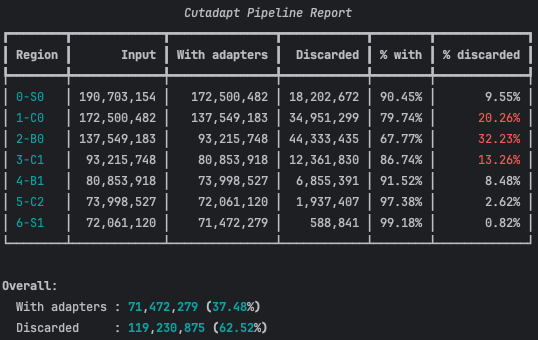
\includegraphics[width=\textwidth]{figures/qc-poor-selection-report.png}
\caption{Example report for a poor selection with only 37\% read retention. The report highlights the problematic region where more than 10\% of the reads are lost during codon assignment, which typically indicates a barcode-definition mismatch, low-quality reads, or an unexpected sequence architecture.}
\label{fig:figure4}
\end{figure}

\begin{figure}[H]
\centering
%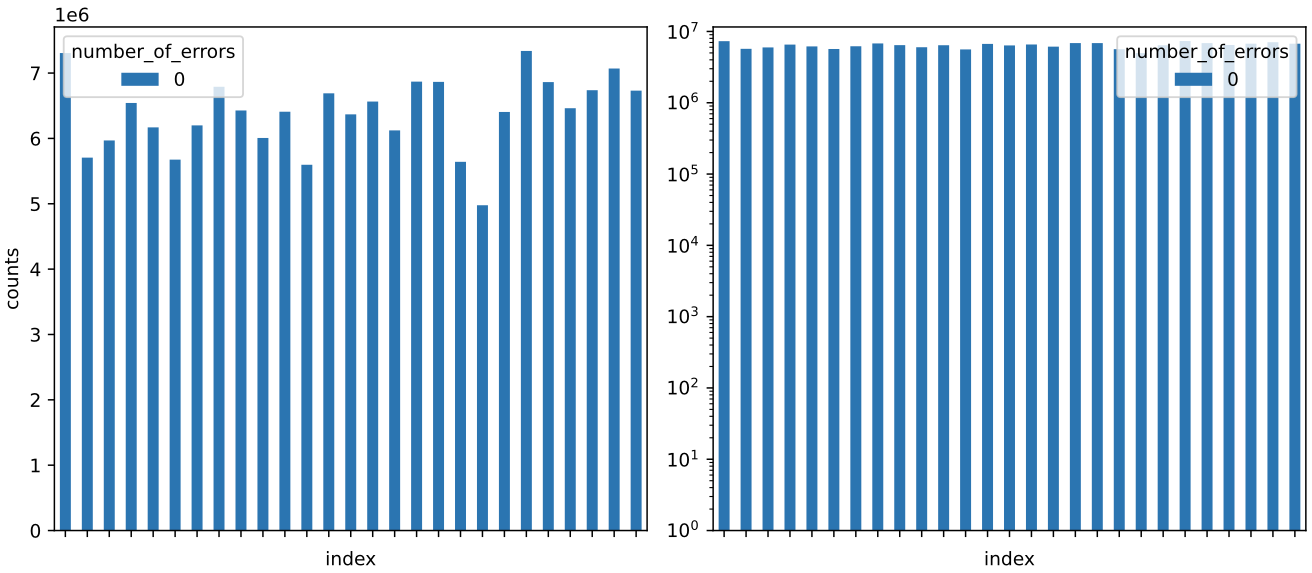
\includegraphics[width=\textwidth]{figures/qc-stacked-barplots.png}
%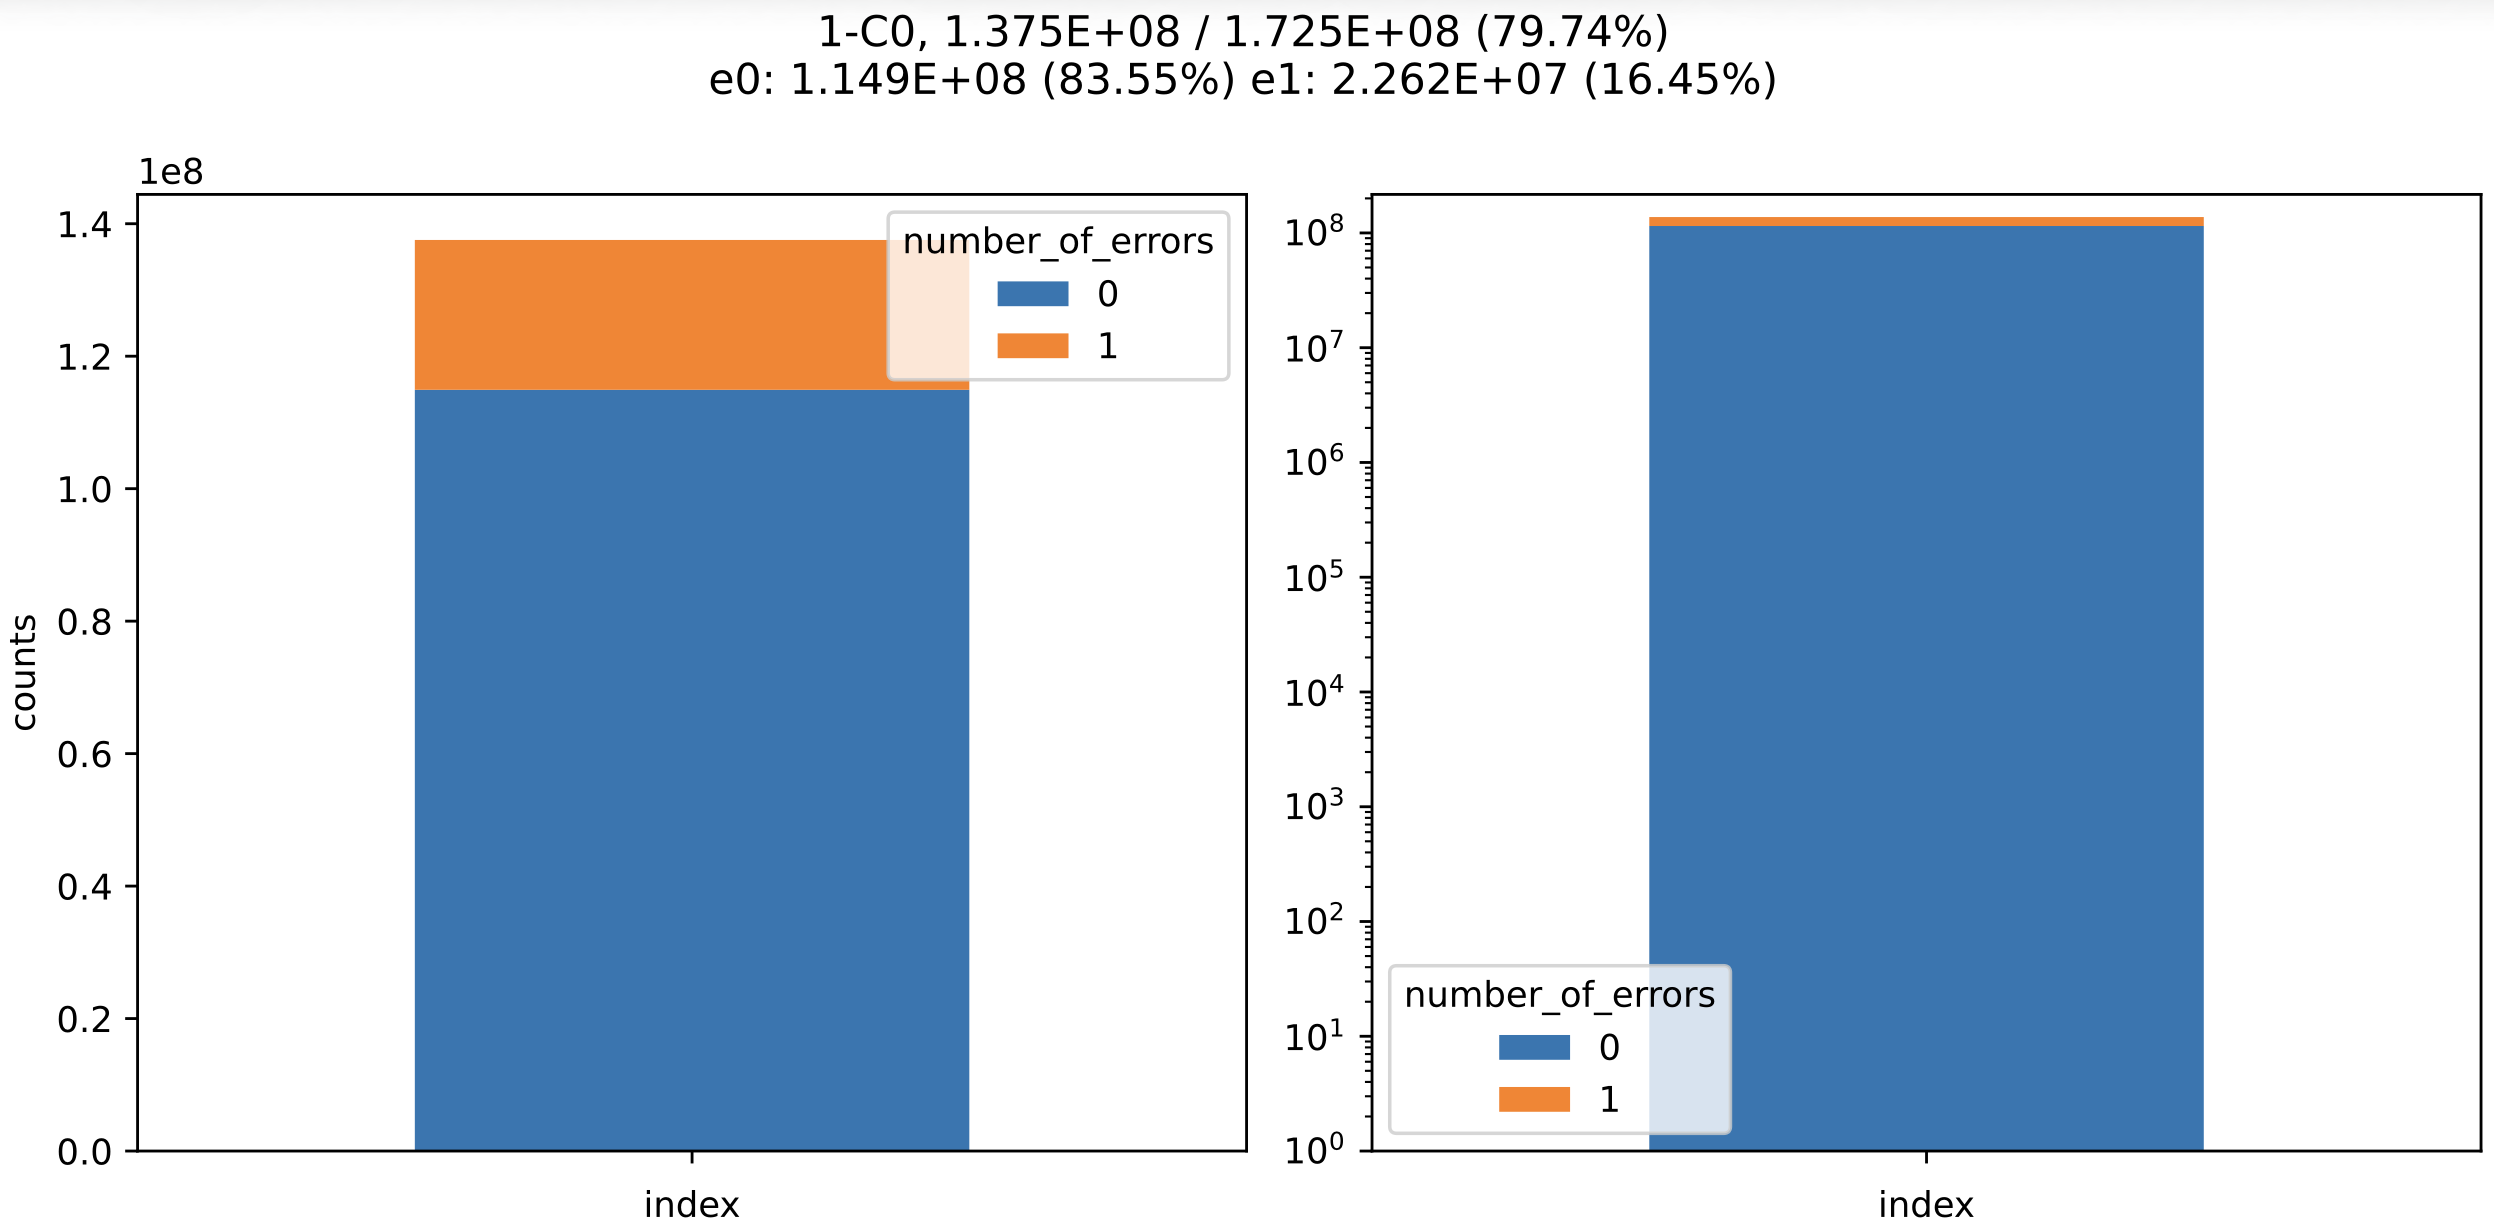
\includegraphics[width=\textwidth]{figures/qc-stacked-barplots-with-errors.png}
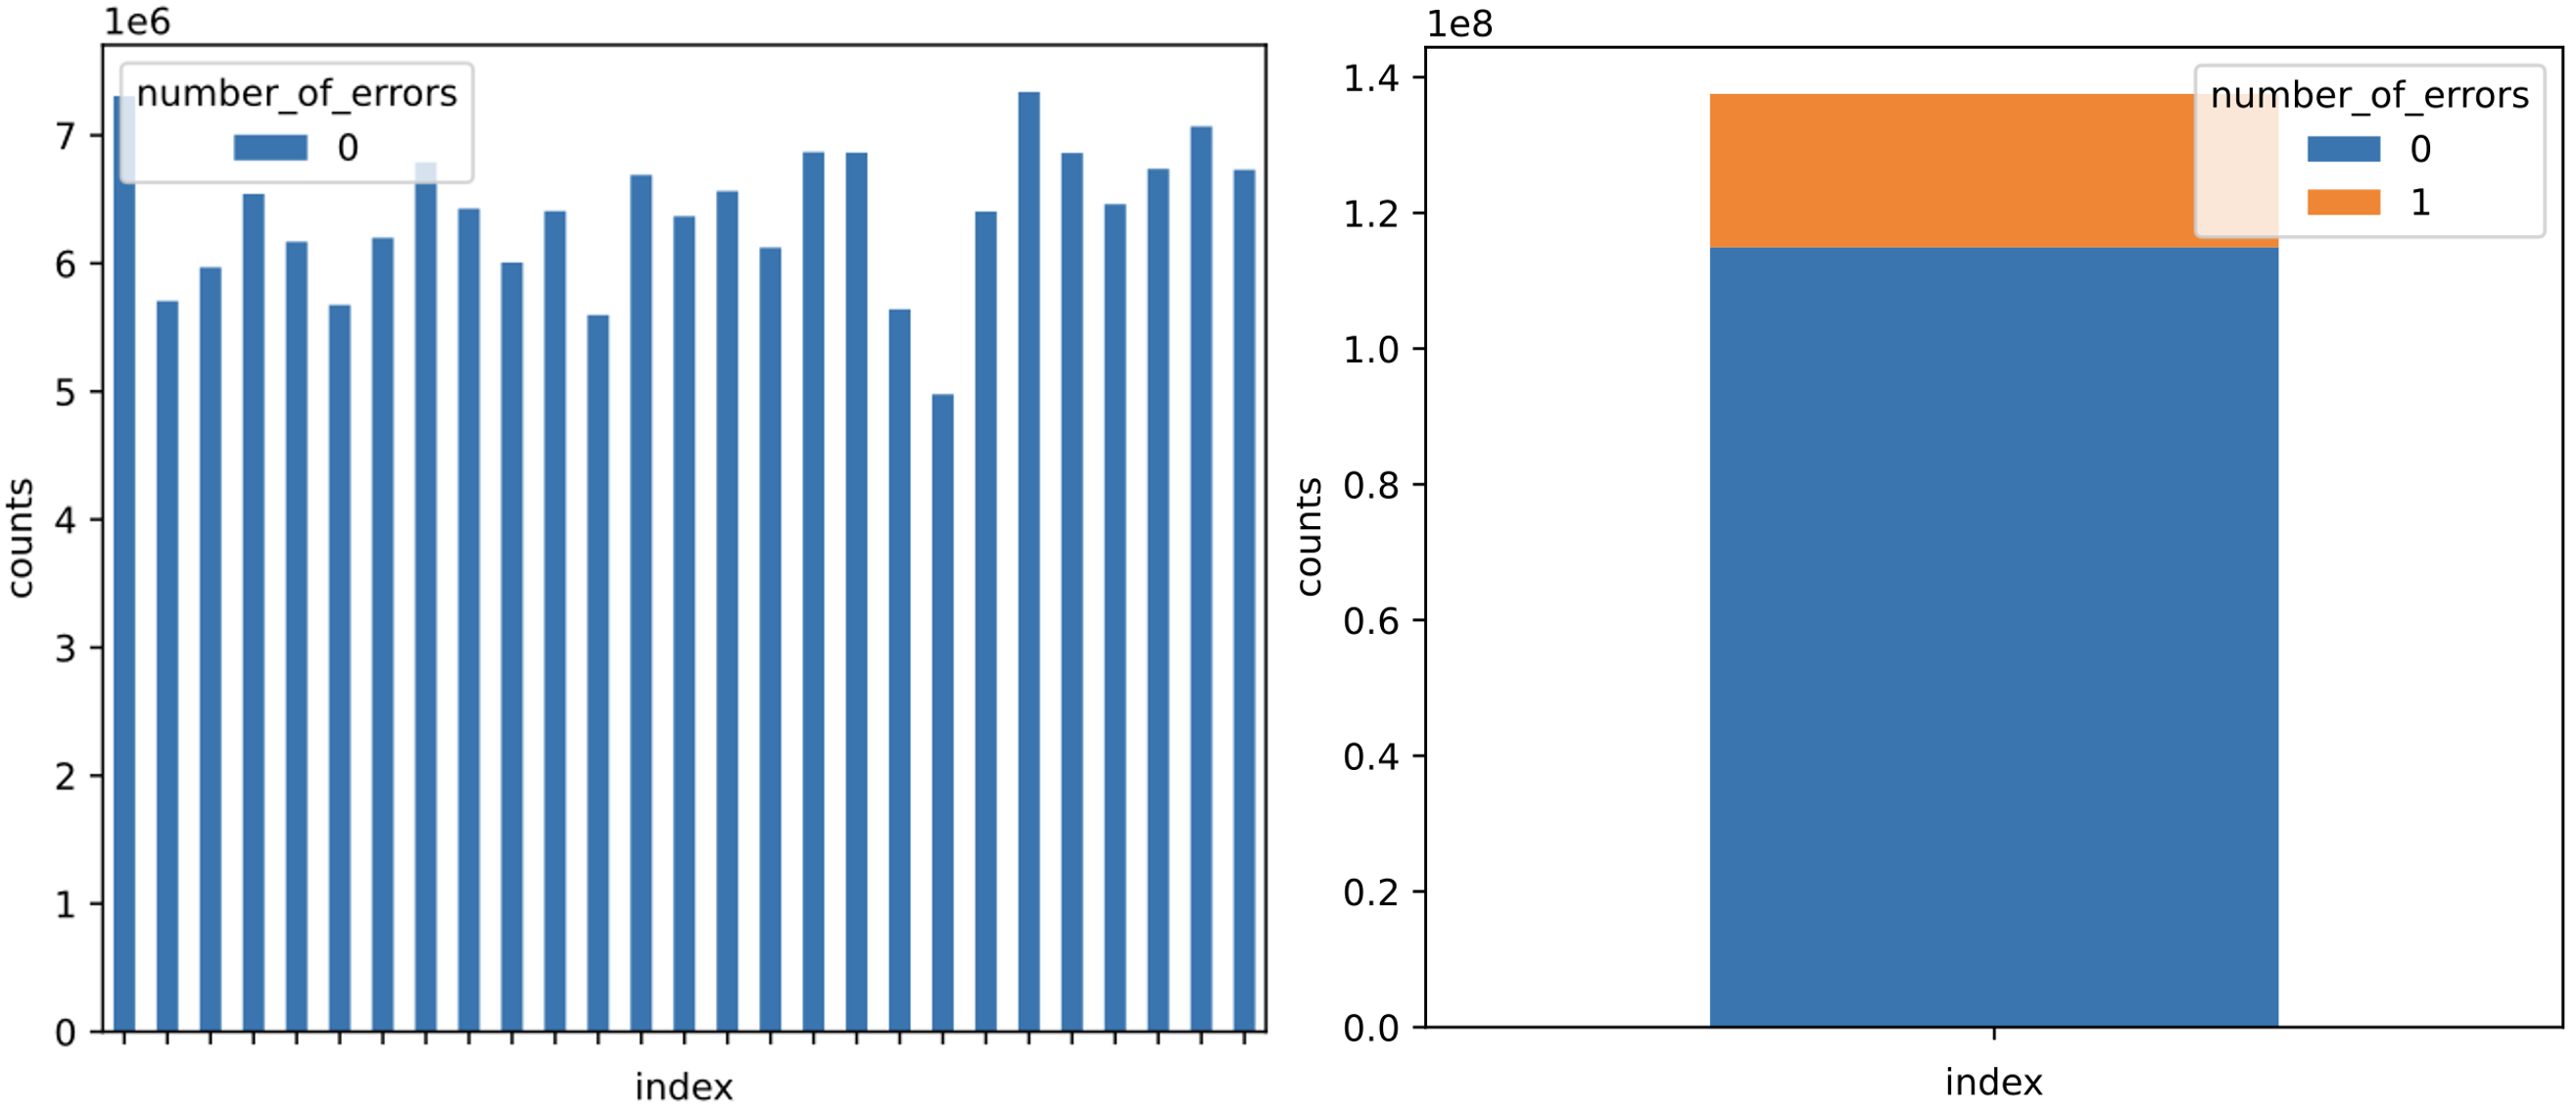
\includegraphics[width=\textwidth]{figures/qc-stacked-barplot-composite.png}
\caption{Quality-control plots showing log-transformed read counts for barcode and constant-region sequences after demultiplexing. The left panel displays the number of reads mapped to building block 0 (BB0) barcode indices, while the right panel shows the number of reads mapped to the constant region 0 index. For the barcode region, exact matching was required, and therefore all mapped reads have 0 sequencing errors. For the constant region, up to one sequencing error was permitted during matching. Reads matching exactly are shown in blue, whereas reads matching with one sequencing error are shown in orange. Strong dropout of individual barcode indices or an increased proportion of one-error matches may indicate issues with oligonucleotide synthesis, sequencing quality, or library preparation.}
\label{fig:figure5}
\end{figure}

\newpage

\protocolstep{12}{Process demultiplexing results into count tables}

Once the quality-control inspection is satisfactory, aggregate the demultiplexed reads into selection-level count tables: 

\begin{lstlisting}
# Process demultiplexing output and generate count tables
delt-hit demultiplex process --config_path=$CONFIG_PATH

# Also export flattened per-selection count files
delt-hit demultiplex process --config_path=$CONFIG_PATH --as_files=True

delt-hit demultiplex process --config_path=$CONFIG_PATH --as_files=True --sort_by_counts=False
\end{lstlisting}

<PAUSE POINT> The generated count tables for each selection are saved in a standardized format for visualization and enrichment analysis.

\subsection{Phase 3 | Data visualization and interpretation}

\textbf{TIMING:} 10--30 min

<CRITICAL>: This phase demonstrates how demultiplexing results can be visualized in the interactive dashboard. 

\protocolstep{13}{Launch the interactive analysis dashboard}
Launch the interactive dashboard and explore count distributions. Open the local server in a web browser, typically at \url{http://localhost:8050} (see print statement in the terminal). Stop the server with \texttt{Ctrl+C} or by closing the terminal. An example dashboard view is shown in Figure~\ref{fig:figure7}.


\begin{lstlisting}
delt-hit dashboard --config_path=$CONFIG_PATH \
  --counts_path=<name>/selections/<selection_name>/counts.txt

# Dash is running on http://127.0.0.1:8050/  # copy and paste into browser
# * Serving Flask app 'delt_hit.cli.dashboard.api'
# * Debug mode: on
\end{lstlisting}


<CRITICAL> The command accepts counts provided as a \texttt{.txt} file, so custom normalized count tables can also be visualized by passing \texttt{--counts\_path} and, if needed, \texttt{--selection\_name}. Use the default folder hierarchy produced by \texttt{delt-hit demultiplex process}. If a custom \texttt{counts.txt} file is provided, also pass the selection name exactly as specified in the selection sheet.

\begin{figure}[htbp]
\centering
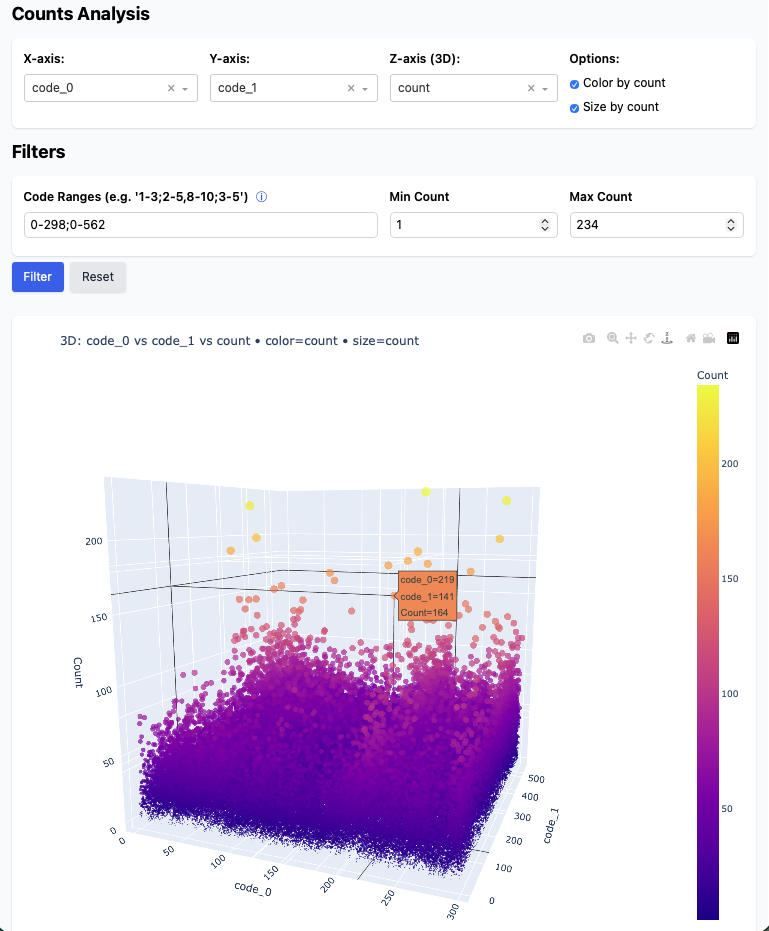
\includegraphics[width=\textwidth]{figures/dashboard.png}
\caption{Interactive dashboard interface for exploring raw count data and experimental metadata. The dashboard provides count-distribution views, filtering controls, and selection-level context to support rapid inspection of demultiplexing outputs before downstream statistical analysis.}
\label{fig:figure7}
\end{figure}

\newpage

\subsection{Phase 4 | Selection enumeration and enrichment analysis}

\textbf{TIMING:} \textless{}1 min
 
<CRITICAL>: This phase generates chemical structures and molecular properties for the top enriched compounds in a selected experiment. 2D representations of the reaction schemes, building blocks and enriched compounds as well as molecular property plots as shown in Figure~\ref{fig:figure2} and Figure~\ref{fig:figure3} can provide visual support for the analysis of selection results. 


\protocolstep{14}{Enumerate top compounds from a selection}
Generate chemical structures for the top enriched compounds in a selected experiment. Visualize the reaction graph to verify the chemical structure of library components.

\begin{lstlisting}
delt-hit visualize enumerate --config_path=$CONFIG_PATH
\end{lstlisting}

Enumerate the \texttt{top\_n} compounds by count for the selected experiment. 

\begin{lstlisting}
delt-hit library enumerate \
  --config_path=$CONFIG_PATH \
  --counts_path=<name>/selections/<selection_name>/counts.txt \
  --top_n=<top_n> \
  --library_name=<library_name>
\end{lstlisting}


\begin{figure}[htbp]
\centering
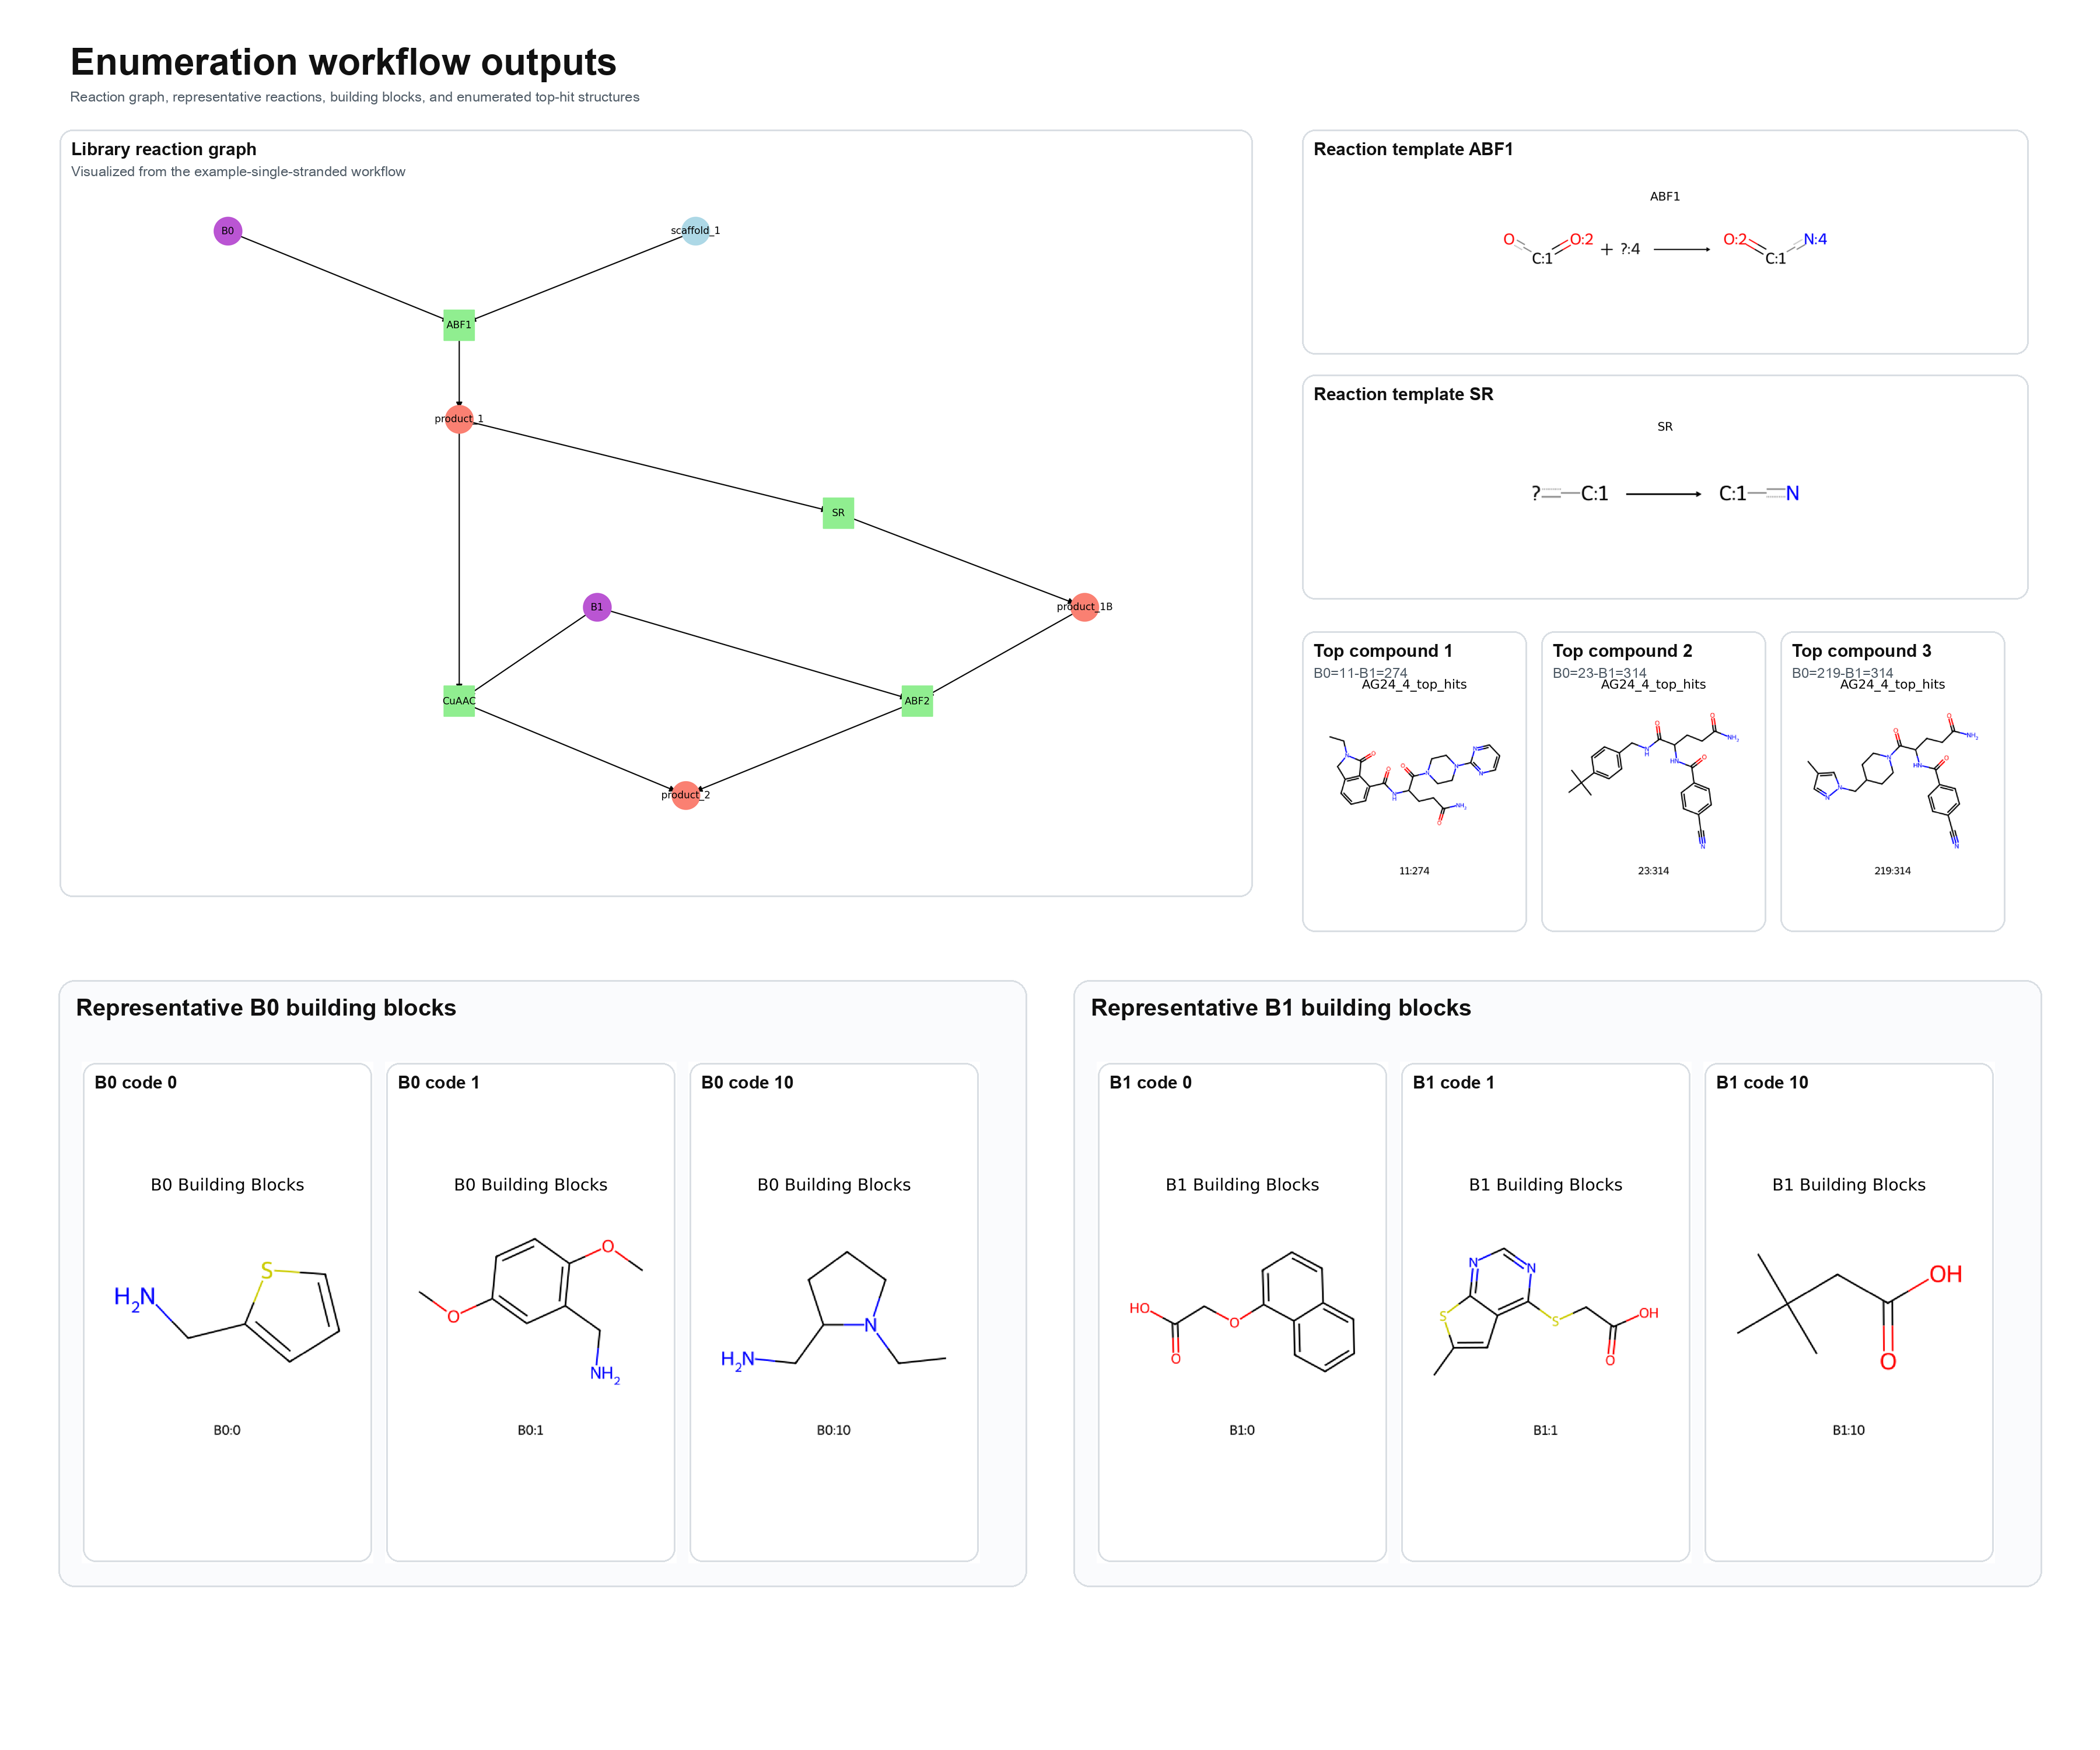
\includegraphics[width=\textwidth]{figures/enumeration-summary.png}
\caption{Composite summary of the enumeration visualization command outputs from the single-display example workflow. The main panel shows the library reaction graph, alongside representative reaction templates and example \texttt{B0} and \texttt{B1} building blocks generated during selection-focused library enumeration.}
\label{fig:figure2}
\end{figure}

<CRITICAL>: Library enumeration requires advanced knowledge of SMIRKS, and library-specific adjustments are often necessary.

\textbf{$\blacklozenge$ Troubleshooting}

\newpage

\protocolstep{15}{Visualize and calculate molecular properties of top hits}

Visualize the chemical structure of the most observed compounds:

\begin{lstlisting}
delt-hit visualize library --config_path=$CONFIG_PATH --library_name=<library_name>
\end{lstlisting}

Calculate molecular descriptors for chemical-space characterization:

\begin{lstlisting}
delt-hit library properties --config_path=$CONFIG_PATH --library_name=<library_name>
\end{lstlisting}


\begin{figure}[H]
\centering
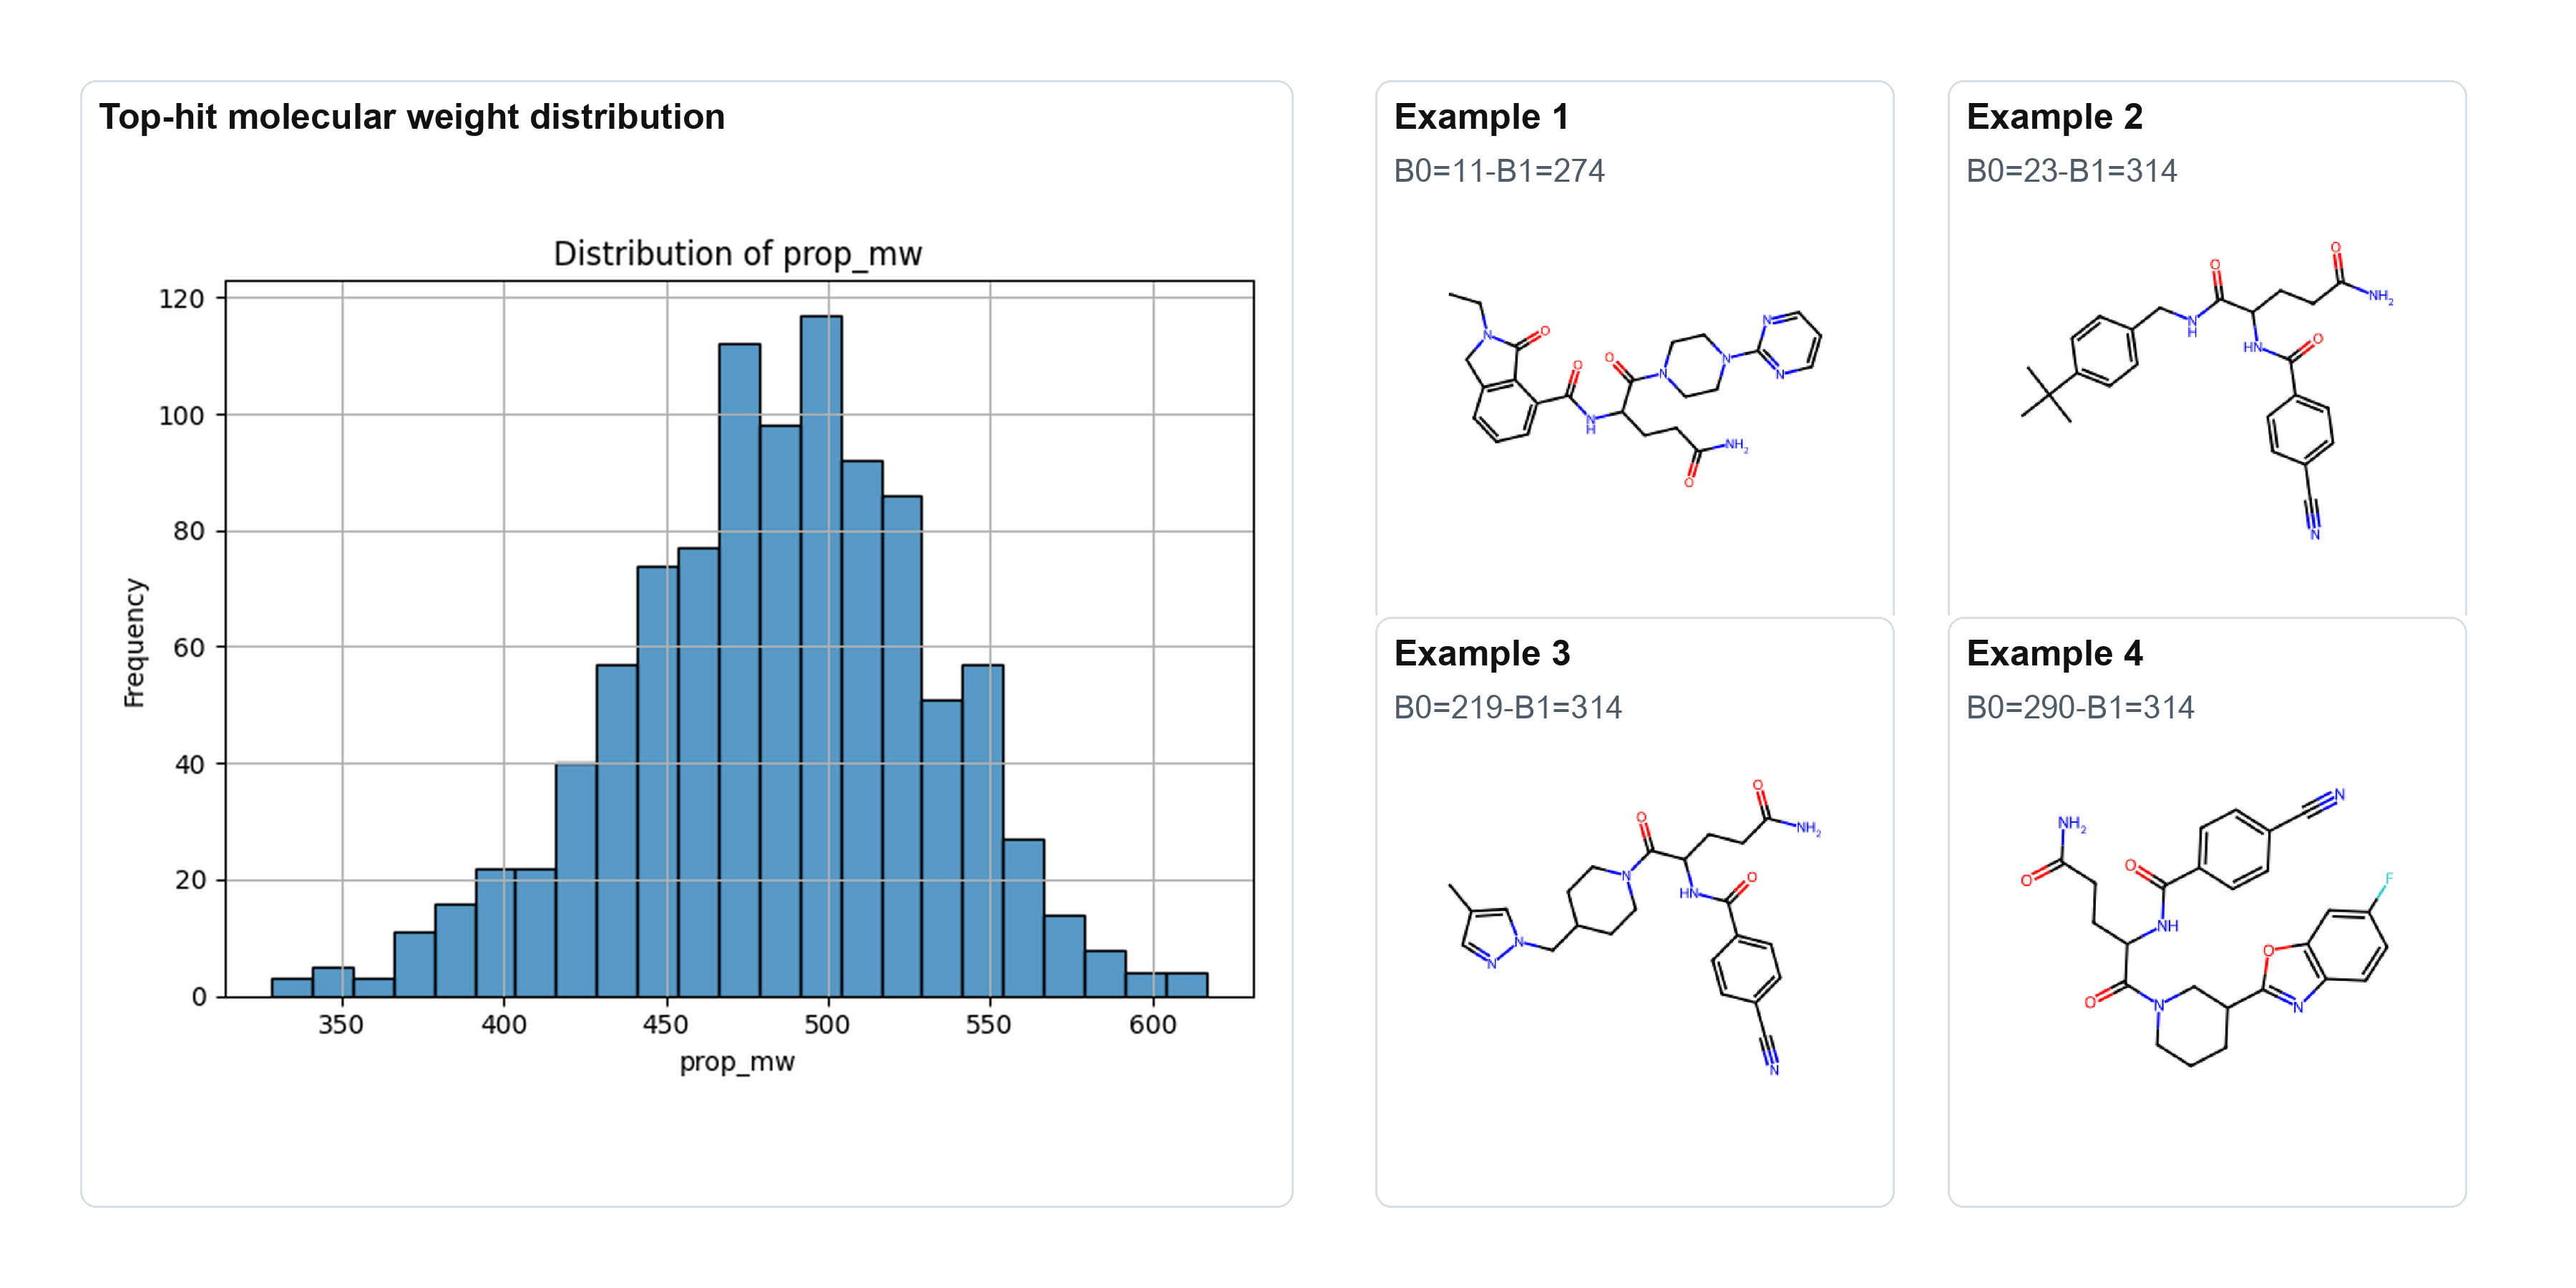
\includegraphics[width=\textwidth]{figures/top-hit-properties-and-structures.png}
\caption{Molecular property and structure summary for the enumerated \texttt{AG24\_4\_top\_hits} collection. The left panel shows the molecular-weight distribution from the example output, and the right panels show four representative structure renderings produced by \texttt{delt-hit visualize library}.}
\label{fig:figure3}
\end{figure}


\subsection{Phase 5 | Statistical analysis and hit identification}

\textbf{TIMING:} \textless{}5 min

<CRITICAL>: This phase identifies enriched library members by comparing selection conditions using established statistical methods.

\protocolstep{16}{Define statistical comparisons}

Using the information from the selection sheet, create a dedicated YAML configuration file that specifies which selections to compare. Comparisons across different selection runs and runs derived from multiple sequencing files are supported. Following the template below, organize the file as a list of \texttt{experiments}, where each experiment defines one named comparison and contains a \texttt{selections} list. Each selection entry specifies the selection name, the corresponding \texttt{counts\_path}, and a \texttt{group} label indicating whether that selection belongs to the control or condition set for the comparison. An example for the single-display workflow (see Box~2) is given below for orientation. 


\begin{lstlisting}
# analysis.yaml -- general structure
experiments:
- name: <experiment_name>        # referenced as --name in commands
  selections:
    - name: <selection_name>
      counts_path: <name>/selections/<selection_name>/counts.txt
      group: control             # or "condition"
    - ...
\end{lstlisting}

Example for the single-display workflow (see Box~2):

\begin{lstlisting}
# analysis.yaml
experiments:
- name: condition_vs_control
  selections:
    - name: AG24_4
      counts_path: campaign/selections/AG24_4/counts.txt
      group: control
    - name: AG24_5
      counts_path: campaign/selections/AG24_5/counts.txt
      group: control
    - name: AG24_6
      counts_path: campaign/selections/AG24_6/counts.txt
      group: control
    - name: AG24_13
      counts_path: campaign/selections/AG24_13/counts.txt
      group: condition
    - name: AG24_14
      counts_path: campaign/selections/AG24_14/counts.txt
      group: condition
    - name: AG24_15
      counts_path: campaign/selections/AG24_15/counts.txt
      group: condition
\end{lstlisting}

\protocolstep{17}{Perform enrichment analysis with statistical methods}
<CRITICAL>: DELT-Hit supports three statistical approaches for identifying enriched compounds. Methods A, B, and C each generate an R script that can be executed directly or adapted further. Use method C for experiments without replicates and any of the three methods for evaluation settings where replicates are available. The generated files report the enrichment score for each compound and, where applicable, method-specific parameters such as log fold change or \textit{P} values.

A. Simple counts method

<CRITICAL>: This method averages counts across replicates within each group and computes a direct enrichment score from the difference between the condition and control groups. While it does not provide formal significance testing, it is useful for comparisons involving replicates as a straightforward ranking approach.

(i) Generate the R script for the counts-based analysis:
\begin{lstlisting}
delt-hit analyse enrichment --analysis_config=<analysis_config> \
  --save_dir=<save_dir> --name=<experiment_name> --method=counts
\end{lstlisting}

(ii) Execute the generated R script:
\begin{lstlisting}
Rscript --vanilla <save_dir>/counts/<experiment_name>/enrichment_counts.R
\end{lstlisting}


B. edgeR method

<CRITICAL>: This method applies RNA-seq-derived statistical modeling with empirical Bayes shrinkage, reports false-discovery-rate-corrected \textit{P} values, and provides normalized count tables for each selection. Use it alongside enrichment ranking as a significance-annotation layer, when replicates are available. An exemplary output for this method is given in Table~\ref{tab:table12}.

(i) Generate the R script for edgeR statistical analysis:
\begin{lstlisting}
delt-hit analyse enrichment --analysis_config=<analysis_config> \
  --save_dir=<save_dir> --name=<experiment_name> --method=edgeR
\end{lstlisting}

(ii) Execute the generated R script:
\begin{lstlisting}
Rscript --vanilla <save_dir>/edgeR/<experiment_name>/enrichment_edgeR.R
\end{lstlisting}


C. Normalized z-score method

<CRITICAL>: This method computes the per-compound score for an individual selection following Faver et al.\cite{faver_quantitativecomparisonenrichment_2019} and can be used for experiments without replicates. The generated output contains both the raw \texttt{z\_score} and the depth-normalized \texttt{norm\_z\_score}, defined as $z\_score / \sqrt{n}$ and used for ranking. 

(i) Generate the R script for normalized z-score analysis:
\begin{lstlisting}
delt-hit analyse enrichment --config_path=$CONFIG_PATH \
  --counts=<name>/selections/<selection_name>/counts.txt \
  --save_dir=<save_dir> --name=<selection_name> --method=z_score
\end{lstlisting}

(ii) Execute the generated R script:
\begin{lstlisting}
Rscript --vanilla <save_dir>/z_score/<selection_name>/enrichment_z_score.R
\end{lstlisting}


\textbf{$\blacklozenge$ Troubleshooting}


<CRITICAL> Guidelines for result interpretation are given below. Always examine replicate correlation plots to verify data quality before interpreting hit lists. Poor correlation may indicate technical problems or batch effects. 

\begin{itemize}
  \item Higher enrichment scores indicate stronger enrichment
  \item Some methods additionally report a log fold change relative to a control; LogFC \textgreater{} 0 corresponds to enrichment relative to the control
  \item FDR \textless{} 0.05 indicates statistically significant enrichment for methods that report adjusted \textit{P} values
  \item High replicate correlation ($R^2 > 0.7$) indicates good experimental consistency
\end{itemize}


% BEGIN flattened input: tables/edger-hits
\begin{table}[htbp]
\centering
\caption{Hit identification by edgeR. Shown compounds are for FDR\textless{}0.05 and sorted by logFC to identify the top hits.}
\label{tab:table12}
\begin{tabular}{lllllll}
\toprule
code\_1 & code\_2 & logFC & logCPM & LR & PValue & FDR \\
\midrule
94 & 472 & 9.76658103 & 4.65399379 & 140.973181 & 1.63E-32 & 2.99E-29 \\
94 & 337 & 9.52452422 & 4.41931582 & 128.115071 & 1.06E-29 & 9.38E-27 \\
250 & 250 & 9.50138143 & 4.39920396 & 136.048263 & 1.95E-31 & 2.62E-28 \\
250 & 523 & 9.46551754 & 4.36448577 & 134.035088 & 5.37E-31 & 6.34E-28 \\
94 & 364 & 9.29500646 & 4.19806216 & 117.172728 & 2.63E-27 & 1.35E-24 \\
250 & 208 & 9.2845154 & 5.99659857 & 173.194896 & 1.48E-39 & 2.05E-35 \\
250 & 337 & 9.06687397 & 3.98375428 & 115.539372 & 6.00E-27 & 2.80E-24 \\
94 & 341 & 8.99590166 & 3.91723403 & 113.847311 & 1.41E-26 & 6.00E-24 \\
250 & 414 & 8.99240694 & 3.90981012 & 105.694583 & 8.60E-25 & 2.69E-22 \\
250 & 96 & 8.92430743 & 8.02773969 & 203.793994 & 3.10E-46 & 2.36E-41 \\
\bottomrule
\end{tabular}
\end{table}

% END flattened input: tables/edger-hits
\subsection{Phase 6 | Full library enumeration and machine learning representations}

\textbf{TIMING:} 15 min--2 h

<CRITICAL>: This phase performs full-library enumeration and generates molecular representations for downstream machine-learning applications. These steps are optional. When only a focused subset is needed, the filtered-enumeration route in Step~14 usually provides a faster alternative to full-library processing.

\protocolstep{18}{Enumerate the full library}

Generate molecular representations of all library members: 

\begin{lstlisting}
delt-hit library enumerate --config_path=$CONFIG_PATH
\end{lstlisting}

\protocolstep{19}{Calculate molecular properties for the full library}

Compute molecular properties for all enumerated compounds:

\begin{lstlisting}
delt-hit library properties --config_path=$CONFIG_PATH
\end{lstlisting}

\protocolstep{20}{Generate molecular representations for machine learning}

Create standardized chemical representations compatible with common machine-learning frameworks. Two methods tailored for different applications are available. Method A (\texttt{morgan}) generates Morgan circular fingerprints (2048-bit vectors), which are useful for similarity analysis. Method B (\texttt{bert}) generates transformer-based molecular embeddings (768-dimensional vectors) for deep-learning applications.


A. Morgan fingerprints

(i) Generate Morgan fingerprints (approximately 600--1000 compounds/s):
\begin{lstlisting}
delt-hit library represent --method=morgan --config_path=$CONFIG_PATH
\end{lstlisting}

B. BERT embeddings

(i) Generate BERT embeddings (approximately 600--1000 compounds/s):
\begin{lstlisting}
delt-hit library represent --method=bert --config_path=$CONFIG_PATH
\end{lstlisting}

\section{Troubleshooting}
Troubleshooting advice for common issues encountered during DELT-Hit analysis can be found in Table~\ref{tab:troubleshooting}.


% BEGIN flattened input: tables/troubleshooting
\begin{table}[htbp]
\centering
\small
\caption{Common issues and solutions}
\label{tab:troubleshooting}
\begin{tabular}{p{2.0cm}p{3.0cm}p{3.8cm}p{5.6cm}}
\toprule
Step & Problem & Possible Cause & Solution \\
\midrule
Setup~Box1 & \texttt{command not found: conda} & Conda not installed or not initialized in the shell & Install Conda as described in the Experimental Setup section and initialize it in your terminal. On macOS: \path{~/miniconda3/bin/activate}; on Windows: \path{~/miniconda3/etc/profile.d/conda.sh} \\
Setup~Box1 & \texttt{command not found: delt-hit} & Conda environment not activated & Run \texttt{conda activate delt-hit} before executing DELT-Hit commands \\
Setup~Box1 / 18 & R script failures & Missing R packages or R not available & Reinstall R into the conda environment; reinstall packages with \texttt{BiocManager}; verify with \texttt{which R}; R 4.1+ required \\
9 & Command fails with unrecognized arguments & Trailing spaces after \textbackslash{} in multiline commands; mistyped command name & Remove trailing spaces from multiline commands and verify the command name. Use \texttt{delt-hit \textless{}cmd\textgreater{} --help} for accepted arguments \\
9 & Demultiplexing fails: \texttt{No such file or directory} & Trailing whitespace in the file name defined in the Excel configuration sheet & Remove whitespace from the file name and regenerate the configuration with \texttt{delt-hit init} \\
11 & Permission denied for shell scripts & Executable permission not set & Run \texttt{chmod u+x \textless{}script\_name.sh\textgreater{}} before executing the script \\
12 & No mapped reads & Incorrect sequences or inverted barcodes & Validate sequences against the sequencing data \\
12 & Low read retention (\textless{}50\%) & Poor library or amplicon quality & Verify library and amplicon quality, repeat selection and/or sequencing if necessary \\
12 & \texttt{qc/report.txt} does not open & Text editor does not support the file encoding & Display the file in the terminal with \texttt{cat qc/report.txt} \\
15 & Chemical structure errors & Invalid SMILES or incorrect reaction SMIRKS & Validate reaction definitions on a small subset before full enumeration; validate building block structures with RDKit; rerun \texttt{delt-hit library enumerate} with \texttt{--debug=invalid --errors=raise} to stop at the first failing combination and save its reaction graph for inspection \\
18 & Empty hit lists & Statistical thresholds too stringent & Adjust FDR cutoffs (0.1 or 0.2 for exploratory analysis); check replicate consistency \\
18 & Poor replicate correlation & Batch effects or technical variability & Review the selection protocol for consistency; check for contamination \\
\bottomrule
\end{tabular}
\end{table}

% END flattened input: tables/troubleshooting
\subsection{Performance optimization guidelines}
Speed and resource usage can be improved by using SSD storage to reduce I/O bottlenecks and by increasing the \texttt{num\_cores} parameter to parallelize compatible steps. Compressed FASTQ files (\texttt{.gz}) do not primarily accelerate processing, but they reduce disk usage and can simplify storage management for large sequencing datasets.

\subsection{Quality control thresholds}
Suggested quality indicators for demultiplexing are:

\begin{itemize}
  \item Excellent: \textgreater{}90\% initial read retention
  \item Good: 70--90\% initial retention
  \item Acceptable: 50--70\% initial retention
  \item Poor: \textless{}50\% retention (requires troubleshooting)
\end{itemize}
Suggested quality indicators for statistical analysis are:

\begin{itemize}
  \item Replicate correlation: $R^2 > 0.7$ for biological replicates and $R^2 > 0.9$ for technical replicates
  \item Positive and negative controls: controls should show the expected behavior
\end{itemize}

\section{Timing}
\label{sec:timing}
Protocol execution times depend on dataset characteristics and computational resources. In particular, some steps scale mainly with the number of sequencing reads, whereas others scale mainly with the number of compounds being enumerated or processed. Table~\ref{tab:table14} separates these two drivers and provides indicative estimates using the recommended hardware configuration (32 GB RAM, 16 CPU cores).

% BEGIN flattened input: tables/timing-estimates
\begin{table}[htbp]
\centering
\caption{Timing estimates for different dataset sizes. For read-dominated steps (especially Steps 10--14), small, medium, and large correspond approximately to \textless{}10 million, 10--100 million, and \textgreater{}100 million reads, respectively. For compound-dominated steps (especially Steps 19--21), small, medium, and large correspond approximately to \textless{}500K, 500K--10M, and \textgreater{}10M library compounds, respectively. These estimates assume that the required laboratory protocol details and library-definition inputs, including building block SMILES, reaction definitions to be converted to SMIRKS, code lists, and related metadata, are readily available to the person performing the workflow}
\label{tab:table14}
\begin{tabular}{p{1.7cm}p{4.4cm}p{2.0cm}p{2.0cm}p{2.0cm}}
\toprule
Step(s) & Analysis Phase & Small & Medium & Large \\
\midrule
Setup & Software installation (one-time) & 15 min & 15 min & 15 min \\
1-9 & Project initialization & 15-30 min & 15-60 min & 30-60 min \\
10-13 & Sequence demultiplexing & 10-30 min & 20-120 min & 2-6 h \\
14 & Visualization and interpretation & 5-15 min & 10-30 min & 15-45 min \\
15 & Library enumeration (selection) & \textless{}1 min & \textless{}1 min & \textless{}1 min \\
16 & Property calculation (selection) & \textless{}1 min & \textless{}1 min & \textless{}1 min \\
17-18 & Statistical analysis & \textless{}5 min & \textless{}5 min & \textless{}5 min \\
19 & Library enumeration (full) & \textless{}5 min & 10 min-1 h & \textgreater{}2 h* \\
20 & Property calculation (full) & \textless{}5 min & 10 min-1 h & \textgreater{}2 h* \\
21 & Molecular representation & \textless{}5 min & 10 min-1 h & \textgreater{}2 h \\
1-21 & Total workflow time & 45 min-1.5 h & 1-6.5 h & \textgreater{}8.5 h* \\
\bottomrule
\end{tabular}
\par\smallskip
\begin{minipage}{\textwidth}
\footnotesize
* Potentially not feasible.
\end{minipage}
\end{table}

% END flattened input: tables/timing-estimates

\section{Anticipated results}

\subsection{Project initialization and configuration}
Successful completion of Steps 1--9 yields a validated project folder containing the parsed workbook information in YAML form:

\begin{lstlisting}
campaign/
`---- config.yaml
\end{lstlisting}

The expected result of this phase is a configuration file that correctly captures the experiment sheet, selection design, sequence architecture, constant regions, and any optional chemistry definitions required for later enumeration. The initialization command reports the created path in the terminal (for example, \texttt{Configuration created at <save\_dir>/<name>/config.yaml}), and the generated YAML should be inspected before downstream processing to confirm that all workbook fields were interpreted as intended.

\subsection{Sequence processing and demultiplexing}
Successful demultiplexing produces staged Cutadapt inputs, per-step logs and statistics, quality-control summaries, and per-selection count tables that can be used directly for downstream quality control and enrichment analysis:

\begin{lstlisting}
campaign/
|---- config.yaml
|---- demultiplex/
|   |---- cutadapt_input_files/
|   |   |---- 0-S0.fastq
|   |   |---- ...
|   |   |---- 6-S1.fastq
|   |   `---- demultiplex.sh
|   `---- cutadapt_output_files/
|       |---- 0-S0.cutadapt.json
|       |---- 0-S0.cutadapt.log
|       |---- ...
|       |---- input.fastq.gz
|       |---- out.fastq.gz
|       `---- reads_with_adapters.gz
|---- qc/
|   |---- report.txt
|   |---- hits_0-S0.{parquet,pdf,png}
|   |---- ...
|   `---- hits_6-S1.{parquet,pdf,png}
`---- selections/
    |---- AG24_4/counts.txt
    |---- ...
    `---- AG24_4_counts.txt
\end{lstlisting}

In this phase, the expected outputs include Cutadapt statistics under \texttt{demultiplex/cutadapt\_output\_files/} as \texttt{*.cutadapt.json} files, the mapped-read intermediate file \texttt{reads\_with\_adapters.gz}, selection-level count tables under \texttt{selections/} as \texttt{<selection\_name>/counts.txt}, optional flattened exports as \texttt{<selection\_name>\_counts.txt}, and quality-control outputs such as \texttt{qc/report.txt}, \texttt{qc/hits\_*.parquet}, \texttt{qc/hits\_*.pdf}, and \texttt{qc/hits\_*.png}.

For high-quality datasets, the demultiplexing outputs typically show (i) high read retention across the sequential adapter-matching steps, (ii) barcode coverage across most or all expected building blocks, and (iii) low sequencing-error rates in the retained reads. The corresponding quality-control plots (Figures~\ref{fig:figure4} and \ref{fig:figure5}) provide a practical overview of these trends and help distinguish balanced selections from runs affected by barcode-definition errors, poor read quality, or library-construction problems. The count tables should contain the building-block index columns (\texttt{code\_0}, \texttt{code\_1}, ..., \texttt{code\_N}), the selection identifier, and the observed read count for each recovered compound.

\subsection{Data visualization and interpretation}
Launching the dashboard in Step~13 starts a local web application for interactive review of demultiplexing-derived count tables and associated metadata. The anticipated outcome is not a new persisted analysis file, but an inspectable browser-based view of raw or custom normalized count tables that allows users to compare selections, explore count distributions, and focus on regions of interest before committing to downstream statistical interpretation.

\subsection{Selection-focused library reconstruction}
Selection-focused enumeration produces a chemically interpretable view of the enriched subset for a chosen selection together with auxiliary visualization and property files:

\begin{lstlisting}
campaign/
`---- library/
    |---- AG24_4_top_hits.parquet
    |---- library.parquet
    |---- visualization/
    |   |---- reaction_graph.png
    |   |---- reaction_graph_additional.png
    |   |---- reaction_graph_building_blocks.png
    |   |---- compounds/
    |   |   `---- scaffold_1.png
    |   |---- reactions/
    |   |   |---- ABF1.png
    |   |   |---- ABF2.png
    |   |   |---- CuAAC.png
    |   |   `---- SR.png
    |   |---- building_blocks/
    |   |   |---- B0/
    |   |   |   `---- *.png
    |   |   `---- B1/
    |   |       `---- *.png
    |   `---- libraries/
    |       `---- AG24_4_top_hits/
    |           `---- B0=<id>-B1=<id>.png
    `---- properties/
        |---- AG24_4_top_hits/
        |   |---- properties.parquet
        |   `---- prop_*.png
        `---- library/
            |---- properties.parquet
            `---- prop_*.png
\end{lstlisting}

In this phase, the expected outputs include the selection-focused compound catalog \texttt{library/<library\_name>.parquet}, reaction-graph visualizations (\texttt{reaction\_graph.png}, \texttt{reaction\_graph\_additional.png}, and \texttt{reaction\_graph\_building\_blocks.png}), the descriptor table \texttt{library/properties/<library\_name>/properties.parquet}, per-property plots \texttt{prop\_*.png}, and structure renderings under \texttt{library/visualization/libraries/<library\_name>/}. The reaction graph (Figure~\ref{fig:figure2}) should confirm that the library architecture and reaction order were translated correctly from the workbook definition. For the single-display example workflow, the molecular-weight distribution and representative top-hit renderings shown in Figure~\ref{fig:figure3} provide a concise view of the resulting chemical space.

\subsection{Statistical analysis and hit identification}
The example workflow contains outputs for multiple enrichment modes, including count-based comparisons, edgeR-based analysis, and normalized z-score-based ranking:

\begin{lstlisting}
campaign/
|---- analysis/
|   |---- counts/
|   |   `---- condition_vs_control/
|   |       |---- samples.csv
|   |       |---- data.csv
|   |       |---- enrichment_counts.R
|   |       |---- stats.csv
|   |       |---- hits.csv
|   |       |---- condition.csv
|   |       |---- control.csv
|   |       `---- correlation_{condition,control}.png
|   |---- edgeR/
|   |   `---- condition_vs_control/
|   |       |---- samples.csv
|   |       |---- data.csv
|   |       |---- enrichment_edgeR.R
|   |       |---- stats.csv
|   |       |---- hits.csv
|   |       |---- AG24_13.csv
|   |       |---- ...
|   |       `---- correlation_{condition,control}.png
|   `---- z_score/
|       |---- AG24_13/
|       |   |---- enrichment_z_score.R
|       |   |---- stats.csv
|       |   `---- hits.csv
|       |---- AG24_14/
|       |   |---- enrichment_z_score.R
|       |   |---- stats.csv
|       |   `---- hits.csv
|       `---- AG24_15/
|           |---- enrichment_z_score.R
|           |---- stats.csv
|           `---- hits.csv
\end{lstlisting}

For each method, the anticipated outputs include an executable analysis script, a full results table (\texttt{stats.csv}), and a ranked hit list (\texttt{hits.csv}); depending on the method, additional normalized tables and replicate-correlation plots are also produced. For the z-score workflow specifically, \texttt{stats.csv} contains both \texttt{z\_score} and \texttt{norm\_z\_score}, and \texttt{hits.csv} is sorted by \texttt{norm\_z\_score}. For a typical comparison, DELT-Hit yields analysis-ready count tables, generated analysis scripts, replicate-correlation plots, and ranked hit lists that can be inspected before interpretation. In well-behaved examples, enriched compounds are separated from the background by a clear dynamic range, whereas unstable controls or inconsistent replicate structure indicate that troubleshooting is needed before biological conclusions are drawn. Troubleshooting advice can be found in Table~\ref{tab:troubleshooting}, and a representative edgeR hit table is shown in Table~\ref{tab:table12}.

\subsection{Full-library enumeration and downstream representations}
Optional full-library processing produces files suitable for cheminformatics and machine-learning workflows:

\begin{lstlisting}
campaign/
|---- library/
|   |---- library.parquet
|   `---- properties/
|       `---- library/
|           |---- properties.parquet
|           `---- prop_*.png
`---- representations/
    |---- morgan.npz
    `---- bert.npz
\end{lstlisting}

These outputs support downstream analysis of the complete library rather than only the compounds identified in the individual selections. In practice, the expected results are (i) a table with calculated compound descriptors and (ii) standardized numerical representations such as \texttt{representations/morgan.npz} and \texttt{representations/bert.npz} that can be used directly for similarity search, clustering, visualization, or machine-learning models built with common Python frameworks.

\section{Data and code availability}

\subsection{Software access and documentation}
DELT-Hit code, supporting material, and source data are archived in persistent repositories. The workflow data and generated outputs are available at \url{https://doi.org/10.5281/zenodo.20447074}, and the DELT-Hit code release used to produce them is available at \url{https://doi.org/10.5281/zenodo.20556531}. DELT-Hit is available under the MIT License:

\begin{itemize}
  \item Workflow data and outputs: \url{https://doi.org/10.5281/zenodo.20447074}
  \item Code release: \url{https://doi.org/10.5281/zenodo.20556531}
  \item Primary repository: \url{https://github.com/DELTechnology/delt-hit}
  \item Installation: {\sloppy\texttt{pip install git+https://git@github.com/DELTechnology/delt-hit.git}\par}
  \item Documentation: user guides, API reference, and tutorials are provided in the repository
  \item Issue tracking: bug reports and support requests can be submitted through GitHub Issues
\end{itemize}

Source data underlying the Supplementary Figures and supplementary comparison and benchmark tables are provided in Supplementary Data 1. The supplementary note set cited throughout the manuscript is collected in the Supplementary Notes document.

\section{Author contributions}
A.M. conceived the project, designed the software architecture, and implemented core algorithms. A.L. created and maintained the configuration files and testing frameworks. L.T. and G.H. implemented core algorithms. A.G. and J.P. performed selection experiments and contributed to result interpretation. L.P. performed software validation and contributed to code refinement. J.S. provided scientific oversight and experimental validation. All authors contributed to manuscript preparation and revision.


\section{Competing interests}
The authors declare no competing financial interests.


\section{Acknowledgments}
We thank the DEL research community for feedback during software development and beta testing. We also acknowledge the developers of Cutadapt, RDKit, edgeR, and other open-source tools used in this workflow, as well as early adopters who helped improve usability and robustness.

\section{Supplementary information}
\textbf{Supplementary Notes}\\
Re-analysis of published datasets, DELT-Hit and DELi workflow comparison, Enrichment scores, Comparison of enrichment score rankings for the Favalli CAIX selection, Advanced reaction-graph configurations

\textbf{Supplementary Data 1}\\
Links to repositories, supplementary data for supplementary figures and tables, SMIRKS reaction templates

\bibliography{../zotero}

\end{document}
